% -----------------------------------------------------------------------------
%                                     HEADER                                    
% -----------------------------------------------------------------------------
\documentclass[a4paper, 10pt]{article}
\usepackage{jheppub}
\usepackage[T1]{fontenc}
\usepackage{colortbl,xcolor,float}
\definecolor{orange}{rgb}{1,0.5,0}
% -----------------------------------------------------------------------------
%                                   COVER PAGE                                  
% -----------------------------------------------------------------------------
\title{{
\includegraphics[scale=.4]{logo.eps}}\ The LaTeX report}

\author{Generated by elijahsheridan on 26 April 2020, 13:54:57}

\abstract{
  This report has been generated automatically
  by {\sc MadAnalysis} 5.\\$~$\\ 
  Please cite:\\ 
  \begin{quote}
    \textbf{E.~Conte, B.~Fuks and G.~Serret},\\ 
    \textit{MadAnalysis 5, A User-Friendly
    Framework for Collider Phenomenology},\\ 
    Comput. Phys. Commun. {\bf 184} (2013) 222-256,\\
    arXiv:1206.1599 [hep-ph].\\ 
  \end{quote}
  To contact us:\\ 
  \begin{quote}
    \textbf{http://madanalysis.irmp.ucl.ac.be}\\
    \textbf{ma5team@iphc.cnrs.fr}\\
  \end{quote}
}

% -----------------------------------------------------------------------------
%                                 BEGIN DOCUMENT                                
% -----------------------------------------------------------------------------
\begin{document}
\maketitle
\flushbottom

% -----------------------------------------------------------------------------
%                                 SECTION Setup                                 
% -----------------------------------------------------------------------------
\newpage
\section{ Setup}

\subsection{ Command history}

\texttt{ma5>\# set directory where running "./\-bin/\-ma5"; set lumi; define the signal significance\\
}
\texttt{ }\texttt{ }\texttt{ma5>set main.currentdir = /\-Users/\-elijahsheridan/\-MG5\_aMC\_v2\_6\_5/\-axion\_pheno/\-madgraph\_data \# need to change this directory path --> exit and type "pwd" to get the path\\
}
\texttt{ }\texttt{ }\texttt{ma5>set main.lumi = 40\\
}
\texttt{ }\texttt{ }\texttt{ma5>set main.fom.formula = 5\\
}
\texttt{ }\texttt{ }\texttt{ma5>set main.fom.x = 0.0\\
}
\texttt{ }\texttt{ }\texttt{ma5>\# import samples --> change the path to the LHE file\\
}
\texttt{ }\texttt{ }\texttt{ma5>import /\-Users/\-elijahsheridan/\-MG5\_aMC\_v2\_6\_5/\-axion\_pheno/\-madgraph\_data/\-axion\_signal/\-axion\_signal\_gurrola\_cuts\_1MeV.lhe.gz as signal\\
}
\texttt{ }\texttt{ }\texttt{ma5>import /\-Users/\-elijahsheridan/\-MG5\_aMC\_v2\_6\_5/\-axion\_pheno/\-madgraph\_data/\-vbf\_diphoton\_background\_data/\-merged\_lhe/\-vbf\_diphoton\_background\_ht\_0\_100\_merged.lhe.gz as bg\_vbf\_0\_100\\
}
\texttt{ }\texttt{ }\texttt{ma5>import /\-Users/\-elijahsheridan/\-MG5\_aMC\_v2\_6\_5/\-axion\_pheno/\-madgraph\_data/\-vbf\_diphoton\_background\_data/\-merged\_lhe/\-vbf\_diphoton\_background\_ht\_100\_200\_merged.lhe.gz as bg\_vbf\_100\_200\\
}
\texttt{ }\texttt{ }\texttt{ma5>import /\-Users/\-elijahsheridan/\-MG5\_aMC\_v2\_6\_5/\-axion\_pheno/\-madgraph\_data/\-vbf\_diphoton\_background\_data/\-merged\_lhe/\-vbf\_diphoton\_background\_ht\_200\_400\_merged.lhe.gz as bg\_vbf\_200\_400\\
}
\texttt{ }\texttt{ }\texttt{ma5>import /\-Users/\-elijahsheridan/\-MG5\_aMC\_v2\_6\_5/\-axion\_pheno/\-madgraph\_data/\-vbf\_diphoton\_background\_data/\-merged\_lhe/\-vbf\_diphoton\_background\_ht\_400\_600\_merged.lhe.gz as bg\_vbf\_400\_600\\
}
\texttt{ }\texttt{ }\texttt{ma5>import /\-Users/\-elijahsheridan/\-MG5\_aMC\_v2\_6\_5/\-axion\_pheno/\-madgraph\_data/\-vbf\_diphoton\_background\_data/\-merged\_lhe/\-vbf\_diphoton\_background\_ht\_600\_800\_merged.lhe.gz as bg\_vbf\_600\_800\\
}
\texttt{ }\texttt{ }\texttt{ma5>import /\-Users/\-elijahsheridan/\-MG5\_aMC\_v2\_6\_5/\-axion\_pheno/\-madgraph\_data/\-vbf\_diphoton\_background\_data/\-merged\_lhe/\-vbf\_diphoton\_background\_ht\_800\_1200\_merged.lhe.gz as bg\_vbf\_800\_1200\\
}
\texttt{ }\texttt{ }\texttt{ma5>import /\-Users/\-elijahsheridan/\-MG5\_aMC\_v2\_6\_5/\-axion\_pheno/\-madgraph\_data/\-vbf\_diphoton\_background\_data/\-merged\_lhe/\-vbf\_diphoton\_background\_ht\_1200\_1600\_merged.lhe.gz as bg\_vbf\_1200\_1600\\
}
\texttt{ }\texttt{ }\texttt{ma5>import /\-Users/\-elijahsheridan/\-MG5\_aMC\_v2\_6\_5/\-axion\_pheno/\-madgraph\_data/\-vbf\_diphoton\_background\_data/\-merged\_lhe/\-vbf\_diphoton\_background\_ht\_1600\_inf\_merged.lhe.gz as bg\_vbf\_1600\_inf\\
}
\texttt{ }\texttt{ }\texttt{ma5>import /\-Users/\-elijahsheridan/\-MG5\_aMC\_v2\_6\_5/\-axion\_pheno/\-madgraph\_data/\-diphoton\_double\_isr\_background\_data/\-merged\_lhe/\-diphoton\_double\_isr\_background\_ht\_0\_100\_merged.lhe.gz as bg\_dip\_0\_100\\
}
\texttt{ }\texttt{ }\texttt{ma5>import /\-Users/\-elijahsheridan/\-MG5\_aMC\_v2\_6\_5/\-axion\_pheno/\-madgraph\_data/\-diphoton\_double\_isr\_background\_data/\-merged\_lhe/\-diphoton\_double\_isr\_background\_ht\_100\_200\_merged.lhe.gz as bg\_dip\_100\_200\\
}
\texttt{ }\texttt{ }\texttt{ma5>import /\-Users/\-elijahsheridan/\-MG5\_aMC\_v2\_6\_5/\-axion\_pheno/\-madgraph\_data/\-diphoton\_double\_isr\_background\_data/\-merged\_lhe/\-diphoton\_double\_isr\_background\_ht\_200\_400\_merged.lhe.gz as bg\_dip\_200\_400\\
}
\texttt{ }\texttt{ }\texttt{ma5>import /\-Users/\-elijahsheridan/\-MG5\_aMC\_v2\_6\_5/\-axion\_pheno/\-madgraph\_data/\-diphoton\_double\_isr\_background\_data/\-merged\_lhe/\-diphoton\_double\_isr\_background\_ht\_400\_600\_merged.lhe.gz as bg\_dip\_400\_600\\
}
\texttt{ }\texttt{ }\texttt{ma5>import /\-Users/\-elijahsheridan/\-MG5\_aMC\_v2\_6\_5/\-axion\_pheno/\-madgraph\_data/\-diphoton\_double\_isr\_background\_data/\-merged\_lhe/\-diphoton\_double\_isr\_background\_ht\_600\_800\_merged.lhe.gz as bg\_dip\_600\_800\\
}
\texttt{ }\texttt{ }\texttt{ma5>import /\-Users/\-elijahsheridan/\-MG5\_aMC\_v2\_6\_5/\-axion\_pheno/\-madgraph\_data/\-diphoton\_double\_isr\_background\_data/\-merged\_lhe/\-diphoton\_double\_isr\_background\_ht\_800\_1200\_merged.lhe.gz as bg\_dip\_800\_1200\\
}
\texttt{ }\texttt{ }\texttt{ma5>import /\-Users/\-elijahsheridan/\-MG5\_aMC\_v2\_6\_5/\-axion\_pheno/\-madgraph\_data/\-diphoton\_double\_isr\_background\_data/\-merged\_lhe/\-diphoton\_double\_isr\_background\_ht\_1200\_1600\_merged.lhe.gz as bg\_dip\_1200\_1600\\
}
\texttt{ }\texttt{ }\texttt{ma5>import /\-Users/\-elijahsheridan/\-MG5\_aMC\_v2\_6\_5/\-axion\_pheno/\-madgraph\_data/\-diphoton\_double\_isr\_background\_data/\-merged\_lhe/\-diphoton\_double\_isr\_background\_ht\_1600\_inf\_merged.lhe.gz as bg\_dip\_1600\_inf\\
}
\texttt{ }\texttt{ }\texttt{ma5>\# define bg and signal samples\\
}
\texttt{ }\texttt{ }\texttt{ma5>set signal.type = signal\\
}
\texttt{ }\texttt{ }\texttt{ma5>set bg\_vbf\_0\_100.type = background\\
}
\texttt{ }\texttt{ }\texttt{ma5>set bg\_vbf\_100\_200.type = background\\
}
\texttt{ }\texttt{ }\texttt{ma5>set bg\_vbf\_200\_400.type  = background\\
}
\texttt{ }\texttt{ }\texttt{ma5>set bg\_vbf\_400\_600.type  = background\\
}
\texttt{ }\texttt{ }\texttt{ma5>set bg\_vbf\_600\_800.type  = background\\
}
\texttt{ }\texttt{ }\texttt{ma5>set bg\_vbf\_800\_1200.type  = background\\
}
\texttt{ }\texttt{ }\texttt{ma5>set bg\_vbf\_1200\_1600.type  = background\\
}
\texttt{ }\texttt{ }\texttt{ma5>set bg\_vbf\_1600\_inf.type = background\\
}
\texttt{ }\texttt{ }\texttt{ma5>set bg\_dip\_0\_100.type = background\\
}
\texttt{ }\texttt{ }\texttt{ma5>set bg\_dip\_100\_200.type = background\\
}
\texttt{ }\texttt{ }\texttt{ma5>set bg\_dip\_200\_400.type = background\\
}
\texttt{ }\texttt{ }\texttt{ma5>set bg\_dip\_400\_600.type = background\\
}
\texttt{ }\texttt{ }\texttt{ma5>set bg\_dip\_600\_800.type = background\\
}
\texttt{ }\texttt{ }\texttt{ma5>set bg\_dip\_800\_1200.type = background\\
}
\texttt{ }\texttt{ }\texttt{ma5>set bg\_dip\_1200\_1600.type = background\\
}
\texttt{ }\texttt{ }\texttt{ma5>set bg\_dip\_1600\_inf.type = background\\
}
\texttt{ }\texttt{ }\texttt{ma5>\# a jet can be from a light quark or b quark\\
}
\texttt{ }\texttt{ }\texttt{ma5>define jets = j\\
}
\texttt{ }\texttt{ }\texttt{ma5>define e = e+ e-\\
}
\texttt{ }\texttt{ }\texttt{ma5>define mu = mu+ mu-\\
}
\texttt{ }\texttt{ }\texttt{ma5>define ta = ta+ ta-\\
}
\texttt{ }\texttt{ }\texttt{ma5>define lept = e mu ta\\
}
\texttt{ }\texttt{ }\texttt{ma5>define ax = 9000005\\
}
\texttt{ }\texttt{ }\texttt{ma5>\# define which plots to make\\
}
\texttt{ }\texttt{ }\texttt{ma5>plot PT(jets[1])\\
}
\texttt{ }\texttt{ }\texttt{ma5>plot ETA(jets[1])\\
}
\texttt{ }\texttt{ }\texttt{ma5>plot PHI(jets[1])\\
}
\texttt{ }\texttt{ }\texttt{ma5>plot PT(jets[2])\\
}
\texttt{ }\texttt{ }\texttt{ma5>plot ETA(jets[2])\\
}
\texttt{ }\texttt{ }\texttt{ma5>plot PHI(jets[2])\\
}
\texttt{ }\texttt{ }\texttt{ma5>plot DELTAR(jets[1], jets[2])\\
}
\texttt{ }\texttt{ }\texttt{ma5>plot M(jets[1] jets[2])\\
}
\texttt{ }\texttt{ }\texttt{ma5>plot sdETA(jets[1] jets[2])\\
}
\texttt{ }\texttt{ }\texttt{ma5>plot M(a[1] a[2])\\
}
\texttt{ }\texttt{ }\texttt{ma5>plot PT(a[1])\\
}
\texttt{ }\texttt{ }\texttt{ma5>plot PT(a[2])\\
}
\texttt{ }\texttt{ }\texttt{ma5>plot THT\\
}
\texttt{ }\texttt{ }\texttt{ma5>plot MET\\
}
\texttt{ }\texttt{ }\texttt{ma5>plot TET\\
}
\texttt{ }\texttt{ }\texttt{ma5>\#set the plot/\-graph parameters\\
}
\texttt{ }\texttt{ }\texttt{ma5>set selection[1].xmin = 0\\
}
\texttt{ }\texttt{ }\texttt{ma5>set selection[1].xmax = 2000\\
}
\texttt{ }\texttt{ }\texttt{ma5>set selection[1].nbins = 200\\
}
\texttt{ }\texttt{ }\texttt{ma5>set selection[1].rank = PTordering\\
}
\texttt{ }\texttt{ }\texttt{ma5>set selection[1].titleX = "p\_\{T\}[j\_\{1\}] (GeV)"\\
}
\texttt{ }\texttt{ }\texttt{ma5>set selection[2].xmin = -8\\
}
\texttt{ }\texttt{ }\texttt{ma5>set selection[2].xmax = 8\\
}
\texttt{ }\texttt{ }\texttt{ma5>set selection[2].nbins = 160\\
}
\texttt{ }\texttt{ }\texttt{ma5>set selection[2].rank = PTordering\\
}
\texttt{ }\texttt{ }\texttt{ma5>set selection[2].titleX = "\#eta[j\_\{1\}]"\\
}
\texttt{ }\texttt{ }\texttt{ma5>set selection[3].xmin = -3.2\\
}
\texttt{ }\texttt{ }\texttt{ma5>set selection[3].xmax = 3.2\\
}
\texttt{ }\texttt{ }\texttt{ma5>set selection[3].nbins = 64\\
}
\texttt{ }\texttt{ }\texttt{ma5>set selection[3].rank = PTordering\\
}
\texttt{ }\texttt{ }\texttt{ma5>set selection[3].titleX = "\#phi[j\_\{1\}]"\\
}
\texttt{ }\texttt{ }\texttt{ma5>set selection[4].xmin = 0\\
}
\texttt{ }\texttt{ }\texttt{ma5>set selection[4].xmax = 1000\\
}
\texttt{ }\texttt{ }\texttt{ma5>set selection[4].nbins = 100\\
}
\texttt{ }\texttt{ }\texttt{ma5>set selection[4].rank = PTordering\\
}
\texttt{ }\texttt{ }\texttt{ma5>set selection[4].titleX = "p\_\{T\}[j\_\{2\}] (GeV)"\\
}
\texttt{ }\texttt{ }\texttt{ma5>set selection[5].xmin = -8\\
}
\texttt{ }\texttt{ }\texttt{ma5>set selection[5].xmax = 8\\
}
\texttt{ }\texttt{ }\texttt{ma5>set selection[5].nbins = 160\\
}
\texttt{ }\texttt{ }\texttt{ma5>set selection[5].rank = PTordering\\
}
\texttt{ }\texttt{ }\texttt{ma5>set selection[5].titleX = "\#eta[j\_\{2\}]"\\
}
\texttt{ }\texttt{ }\texttt{ma5>set selection[6].xmin = -3.2\\
}
\texttt{ }\texttt{ }\texttt{ma5>set selection[6].xmax = 3.2\\
}
\texttt{ }\texttt{ }\texttt{ma5>set selection[6].nbins = 64\\
}
\texttt{ }\texttt{ }\texttt{ma5>set selection[6].rank = PTordering\\
}
\texttt{ }\texttt{ }\texttt{ma5>set selection[6].titleX = "\#phi[j\_\{2\}]"\\
}
\texttt{ }\texttt{ }\texttt{ma5>set selection[7].xmin = 0\\
}
\texttt{ }\texttt{ }\texttt{ma5>set selection[7].xmax = 15\\
}
\texttt{ }\texttt{ }\texttt{ma5>set selection[7].nbins = 75\\
}
\texttt{ }\texttt{ }\texttt{ma5>set selection[7].rank = PTordering\\
}
\texttt{ }\texttt{ }\texttt{ma5>set selection[7].titleX = "\#DeltaR[j\_\{1\},j\_\{2\}]"\\
}
\texttt{ }\texttt{ }\texttt{ma5>set selection[8].xmin = 0\\
}
\texttt{ }\texttt{ }\texttt{ma5>set selection[8].xmax = 8000\\
}
\texttt{ }\texttt{ }\texttt{ma5>set selection[8].nbins = 160\\
}
\texttt{ }\texttt{ }\texttt{ma5>set selection[8].rank = PTordering\\
}
\texttt{ }\texttt{ }\texttt{ma5>set selection[8].titleX = "M[j\_\{1\},j\_\{2\}] (GeV)"\\
}
\texttt{ }\texttt{ }\texttt{ma5>set selection[9].xmin = -15\\
}
\texttt{ }\texttt{ }\texttt{ma5>set selection[9].xmax = 15\\
}
\texttt{ }\texttt{ }\texttt{ma5>set selection[9].titleX = "\#Delta\#eta(j\_\{1\},j\_\{2\})"\\
}
\texttt{ }\texttt{ }\texttt{ma5>set selection[10].xmin = 0\\
}
\texttt{ }\texttt{ }\texttt{ma5>set selection[10].xmax = 4000\\
}
\texttt{ }\texttt{ }\texttt{ma5>set selection[10].nbins = 400\\
}
\texttt{ }\texttt{ }\texttt{ma5>set selection[10].rank = PTordering\\
}
\texttt{ }\texttt{ }\texttt{ma5>set selection[10].titleX = "M[a\_\{1\},a\_\{2\}] (GeV)"\\
}
\texttt{ }\texttt{ }\texttt{ma5>set selection[11].xmin = 0\\
}
\texttt{ }\texttt{ }\texttt{ma5>set selection[11].xmax = 2000\\
}
\texttt{ }\texttt{ }\texttt{ma5>set selection[11].nbins = 80\\
}
\texttt{ }\texttt{ }\texttt{ma5>set selection[11].rank = PTordering\\
}
\texttt{ }\texttt{ }\texttt{ma5>set selection[11].titleX = "p\_\{T\}[a\_\{1\}]"\\
}
\texttt{ }\texttt{ }\texttt{ma5>set selection[12].xmin = 0\\
}
\texttt{ }\texttt{ }\texttt{ma5>set selection[12].xmax = 2000\\
}
\texttt{ }\texttt{ }\texttt{ma5>set selection[12].nbins = 400\\
}
\texttt{ }\texttt{ }\texttt{ma5>set selection[12].rank = PTordering\\
}
\texttt{ }\texttt{ }\texttt{ma5>set selection[12].titleX = "p\_\{T\}[a\_\{2\}] (GeV)"\\
}
\texttt{ }\texttt{ }\texttt{ma5>set selection[13].xmin = 0\\
}
\texttt{ }\texttt{ }\texttt{ma5>set selection[13].xmax = 4000\\
}
\texttt{ }\texttt{ }\texttt{ma5>set selection[13].nbins = 80\\
}
\texttt{ }\texttt{ }\texttt{ma5>set selection[13].rank = PTordering\\
}
\texttt{ }\texttt{ }\texttt{ma5>set selection[13].titleX = "THT"\\
}
\texttt{ }\texttt{ }\texttt{ma5>set selection[14].xmin = 0\\
}
\texttt{ }\texttt{ }\texttt{ma5>set selection[14].xmax = 1000\\
}
\texttt{ }\texttt{ }\texttt{ma5>set selection[14].nbins = 200\\
}
\texttt{ }\texttt{ }\texttt{ma5>set selection[14].rank = PTordering\\
}
\texttt{ }\texttt{ }\texttt{ma5>set selection[14].titleX = "MET"\\
}
\texttt{ }\texttt{ }\texttt{ma5>set selection[15].xmin = 0\\
}
\texttt{ }\texttt{ }\texttt{ma5>set selection[15].xmax = 8000\\
}
\texttt{ }\texttt{ }\texttt{ma5>set selection[15].nbins = 80\\
}
\texttt{ }\texttt{ }\texttt{ma5>set selection[15].rank = PTordering\\
}
\texttt{ }\texttt{ }\texttt{ma5>set selection[15].titleX = "TET"\\
}
\texttt{ }\texttt{ }\texttt{ma5>submit no\_cuts\\
}
\texttt{ }\texttt{ }\subsection{ Configuration}

\begin{itemize}
  \item MadAnalysis version 1.6.33 (2017/\-11/\-20).
   \item Histograms given for an integrated luminosity of \textcolor{blue}{40.0}\textcolor{blue}{ fb}$^{\textcolor{blue}{-1}}$\textcolor{blue}{.}
\textcolor{blue}{}
\end{itemize}
% -----------------------------------------------------------------------------
%                                SECTION Datasets                               
% -----------------------------------------------------------------------------
\newpage
\section{ Datasets}

\subsection{ signal}

\begin{itemize}
  \item Samples stored in the directory: \textcolor{blue}{/\-Users/\-elijahsheridan/\-MG5\_aMC\_v2\_6\_5/\-axion\_pheno/\-optimization/\-ma\_scripts} .
   \item Sample consisting of: \textcolor{blue}{signal}  events.
   \item Generated events: \textcolor{blue}{1000000 }  events.
   \item Normalization to the luminosity: \textcolor{blue}{4094}\textcolor{blue}{ +/\-- }\textcolor{blue}{2 }  events.
   \item Ratio (event weight): \textcolor{blue}{0.0041 } .  
 
\end{itemize}
\begin{table}[H]
  \begin{center}
    \begin{tabular}{|m{55.0mm}|m{25.0mm}|m{30.0mm}|m{30.0mm}|}
      \hline
      {\cellcolor{yellow}         Path to the event file}& {\cellcolor{yellow}         Nr. of events}& {\cellcolor{yellow}         Cross section (pb)}& {\cellcolor{yellow}         Negative wgts (\%)}\\
      \hline
      {\cellcolor{white}          /\-Users/\-elijahsheridan/\-MG5\_aMC\_v2\_6\_5/\-axion\_pheno/\-madgraph\_data/\-axion\_signal/\-axion\_signal\_gurrola\_cuts\_1MeV.lhe.gz}& {\cellcolor{white}          1000000}& {\cellcolor{white}          0.102 @ 0.028\%}& {\cellcolor{white}          0.0}\\
\hline
    \end{tabular}
  \end{center}
\end{table}

\subsection{ bg\_vbf\_0\_100}

\begin{itemize}
  \item Samples stored in the directory: \textcolor{blue}{/\-Users/\-elijahsheridan/\-MG5\_aMC\_v2\_6\_5/\-axion\_pheno/\-optimization/\-ma\_scripts} .
   \item Sample consisting of: \textcolor{blue}{background}  events.
   \item Generated events: \textcolor{blue}{1000000 }  events.
   \item Normalization to the luminosity: \textcolor{blue}{12150}\textcolor{blue}{ +/\-- }\textcolor{blue}{24 }  events.
   \item Ratio (event weight): \textcolor{blue}{0.012 } .  
 
\end{itemize}
\begin{table}[H]
  \begin{center}
    \begin{tabular}{|m{55.0mm}|m{25.0mm}|m{30.0mm}|m{30.0mm}|}
      \hline
      {\cellcolor{yellow}         Path to the event file}& {\cellcolor{yellow}         Nr. of events}& {\cellcolor{yellow}         Cross section (pb)}& {\cellcolor{yellow}         Negative wgts (\%)}\\
      \hline
      {\cellcolor{white}          /\-Users/\-elijahsheridan/\-MG5\_aMC\_v2\_6\_5/\-axion\_pheno/\-madgraph\_data/\-vbf\_diphoton\_background\_data/\-merged\_lhe/\-vbf\_diphoton\_background\_ht\_0\_100\_merged.lhe.gz}& {\cellcolor{white}          1000000}& {\cellcolor{white}          0.304 @ 0.19\%}& {\cellcolor{white}          0.0}\\
\hline
    \end{tabular}
  \end{center}
\end{table}

\subsection{ bg\_vbf\_100\_200}

\begin{itemize}
  \item Samples stored in the directory: \textcolor{blue}{/\-Users/\-elijahsheridan/\-MG5\_aMC\_v2\_6\_5/\-axion\_pheno/\-optimization/\-ma\_scripts} .
   \item Sample consisting of: \textcolor{blue}{background}  events.
   \item Generated events: \textcolor{blue}{965662 }  events.
   \item Normalization to the luminosity: \textcolor{blue}{9695}\textcolor{blue}{ +/\-- }\textcolor{blue}{17 }  events.
   \item Ratio (event weight): \textcolor{blue}{0.01 } .  
 
\end{itemize}
\begin{table}[H]
  \begin{center}
    \begin{tabular}{|m{55.0mm}|m{25.0mm}|m{30.0mm}|m{30.0mm}|}
      \hline
      {\cellcolor{yellow}         Path to the event file}& {\cellcolor{yellow}         Nr. of events}& {\cellcolor{yellow}         Cross section (pb)}& {\cellcolor{yellow}         Negative wgts (\%)}\\
      \hline
      {\cellcolor{white}          /\-Users/\-elijahsheridan/\-MG5\_aMC\_v2\_6\_5/\-axion\_pheno/\-madgraph\_data/\-vbf\_diphoton\_background\_data/\-merged\_lhe/\-vbf\_diphoton\_background\_ht\_100\_200\_merged.lhe.gz}& {\cellcolor{white}          965662}& {\cellcolor{white}          0.242 @ 0.17\%}& {\cellcolor{white}          0.0}\\
\hline
    \end{tabular}
  \end{center}
\end{table}

\subsection{ bg\_vbf\_200\_400}

\begin{itemize}
  \item Samples stored in the directory: \textcolor{blue}{/\-Users/\-elijahsheridan/\-MG5\_aMC\_v2\_6\_5/\-axion\_pheno/\-optimization/\-ma\_scripts} .
   \item Sample consisting of: \textcolor{blue}{background}  events.
   \item Generated events: \textcolor{blue}{984165 }  events.
   \item Normalization to the luminosity: \textcolor{blue}{5413}\textcolor{blue}{ +/\-- }\textcolor{blue}{11 }  events.
   \item Ratio (event weight): \textcolor{blue}{0.0055 } .  
 
\end{itemize}
\begin{table}[H]
  \begin{center}
    \begin{tabular}{|m{55.0mm}|m{25.0mm}|m{30.0mm}|m{30.0mm}|}
      \hline
      {\cellcolor{yellow}         Path to the event file}& {\cellcolor{yellow}         Nr. of events}& {\cellcolor{yellow}         Cross section (pb)}& {\cellcolor{yellow}         Negative wgts (\%)}\\
      \hline
      {\cellcolor{white}          /\-Users/\-elijahsheridan/\-MG5\_aMC\_v2\_6\_5/\-axion\_pheno/\-madgraph\_data/\-vbf\_diphoton\_background\_data/\-merged\_lhe/\-vbf\_diphoton\_background\_ht\_200\_400\_merged.lhe.gz}& {\cellcolor{white}          984165}& {\cellcolor{white}          0.135 @ 0.2\%}& {\cellcolor{white}          0.0}\\
\hline
    \end{tabular}
  \end{center}
\end{table}

\subsection{ bg\_vbf\_400\_600}

\begin{itemize}
  \item Samples stored in the directory: \textcolor{blue}{/\-Users/\-elijahsheridan/\-MG5\_aMC\_v2\_6\_5/\-axion\_pheno/\-optimization/\-ma\_scripts} .
   \item Sample consisting of: \textcolor{blue}{background}  events.
   \item Generated events: \textcolor{blue}{1000000 }  events.
   \item Normalization to the luminosity: \textcolor{blue}{986}\textcolor{blue}{ +/\-- }\textcolor{blue}{2 }  events.
   \item Ratio (event weight): \textcolor{blue}{0.00099 } .  
 
\end{itemize}
\begin{table}[H]
  \begin{center}
    \begin{tabular}{|m{55.0mm}|m{25.0mm}|m{30.0mm}|m{30.0mm}|}
      \hline
      {\cellcolor{yellow}         Path to the event file}& {\cellcolor{yellow}         Nr. of events}& {\cellcolor{yellow}         Cross section (pb)}& {\cellcolor{yellow}         Negative wgts (\%)}\\
      \hline
      {\cellcolor{white}          /\-Users/\-elijahsheridan/\-MG5\_aMC\_v2\_6\_5/\-axion\_pheno/\-madgraph\_data/\-vbf\_diphoton\_background\_data/\-merged\_lhe/\-vbf\_diphoton\_background\_ht\_400\_600\_merged.lhe.gz}& {\cellcolor{white}          1000000}& {\cellcolor{white}          0.0247 @ 0.14\%}& {\cellcolor{white}          0.0}\\
\hline
    \end{tabular}
  \end{center}
\end{table}

\subsection{ bg\_vbf\_600\_800}

\begin{itemize}
  \item Samples stored in the directory: \textcolor{blue}{/\-Users/\-elijahsheridan/\-MG5\_aMC\_v2\_6\_5/\-axion\_pheno/\-optimization/\-ma\_scripts} .
   \item Sample consisting of: \textcolor{blue}{background}  events.
   \item Generated events: \textcolor{blue}{1000000 }  events.
   \item Normalization to the luminosity: \textcolor{blue}{252}\textcolor{blue}{ +/\-- }\textcolor{blue}{1 }  events.
   \item Ratio (event weight): \textcolor{blue}{0.00025 } .  
 
\end{itemize}
\begin{table}[H]
  \begin{center}
    \begin{tabular}{|m{55.0mm}|m{25.0mm}|m{30.0mm}|m{30.0mm}|}
      \hline
      {\cellcolor{yellow}         Path to the event file}& {\cellcolor{yellow}         Nr. of events}& {\cellcolor{yellow}         Cross section (pb)}& {\cellcolor{yellow}         Negative wgts (\%)}\\
      \hline
      {\cellcolor{white}          /\-Users/\-elijahsheridan/\-MG5\_aMC\_v2\_6\_5/\-axion\_pheno/\-madgraph\_data/\-vbf\_diphoton\_background\_data/\-merged\_lhe/\-vbf\_diphoton\_background\_ht\_600\_800\_merged.lhe.gz}& {\cellcolor{white}          1000000}& {\cellcolor{white}          0.0063 @ 0.13\%}& {\cellcolor{white}          0.0}\\
\hline
    \end{tabular}
  \end{center}
\end{table}

\subsection{ bg\_vbf\_800\_1200}

\begin{itemize}
  \item Samples stored in the directory: \textcolor{blue}{/\-Users/\-elijahsheridan/\-MG5\_aMC\_v2\_6\_5/\-axion\_pheno/\-optimization/\-ma\_scripts} .
   \item Sample consisting of: \textcolor{blue}{background}  events.
   \item Generated events: \textcolor{blue}{400839 }  events.
   \item Normalization to the luminosity: \textcolor{blue}{114}\textcolor{blue}{ +/\-- }\textcolor{blue}{1 }  events.
   \item Ratio (event weight): \textcolor{blue}{0.00028 } .  
 
\end{itemize}
\begin{table}[H]
  \begin{center}
    \begin{tabular}{|m{55.0mm}|m{25.0mm}|m{30.0mm}|m{30.0mm}|}
      \hline
      {\cellcolor{yellow}         Path to the event file}& {\cellcolor{yellow}         Nr. of events}& {\cellcolor{yellow}         Cross section (pb)}& {\cellcolor{yellow}         Negative wgts (\%)}\\
      \hline
      {\cellcolor{white}          /\-Users/\-elijahsheridan/\-MG5\_aMC\_v2\_6\_5/\-axion\_pheno/\-madgraph\_data/\-vbf\_diphoton\_background\_data/\-merged\_lhe/\-vbf\_diphoton\_background\_ht\_800\_1200\_merged.lhe.gz}& {\cellcolor{white}          400839}& {\cellcolor{white}          0.00287 @ 0.16\%}& {\cellcolor{white}          0.0}\\
\hline
    \end{tabular}
  \end{center}
\end{table}

\subsection{ bg\_vbf\_1200\_1600}

\begin{itemize}
  \item Samples stored in the directory: \textcolor{blue}{/\-Users/\-elijahsheridan/\-MG5\_aMC\_v2\_6\_5/\-axion\_pheno/\-optimization/\-ma\_scripts} .
   \item Sample consisting of: \textcolor{blue}{background}  events.
   \item Generated events: \textcolor{blue}{953803 }  events.
   \item Normalization to the luminosity: \textcolor{blue}{20}\textcolor{blue}{ +/\-- }\textcolor{blue}{1 }  events.
   \item Ratio (event weight): \textcolor{blue}{2.1e-05 } .  
 
\end{itemize}
\begin{table}[H]
  \begin{center}
    \begin{tabular}{|m{55.0mm}|m{25.0mm}|m{30.0mm}|m{30.0mm}|}
      \hline
      {\cellcolor{yellow}         Path to the event file}& {\cellcolor{yellow}         Nr. of events}& {\cellcolor{yellow}         Cross section (pb)}& {\cellcolor{yellow}         Negative wgts (\%)}\\
      \hline
      {\cellcolor{white}          /\-Users/\-elijahsheridan/\-MG5\_aMC\_v2\_6\_5/\-axion\_pheno/\-madgraph\_data/\-vbf\_diphoton\_background\_data/\-merged\_lhe/\-vbf\_diphoton\_background\_ht\_1200\_1600\_merged.lhe.gz}& {\cellcolor{white}          953803}& {\cellcolor{white}          0.000515 @ 0.16\%}& {\cellcolor{white}          0.0}\\
\hline
    \end{tabular}
  \end{center}
\end{table}

\subsection{ bg\_vbf\_1600\_inf}

\begin{itemize}
  \item Samples stored in the directory: \textcolor{blue}{/\-Users/\-elijahsheridan/\-MG5\_aMC\_v2\_6\_5/\-axion\_pheno/\-optimization/\-ma\_scripts} .
   \item Sample consisting of: \textcolor{blue}{background}  events.
   \item Generated events: \textcolor{blue}{270148 }  events.
   \item Normalization to the luminosity: \textcolor{blue}{7}\textcolor{blue}{ +/\-- }\textcolor{blue}{1 }  events.
   \item Ratio (event weight): \textcolor{blue}{2.6e-05 } .  
 
\end{itemize}
\begin{table}[H]
  \begin{center}
    \begin{tabular}{|m{55.0mm}|m{25.0mm}|m{30.0mm}|m{30.0mm}|}
      \hline
      {\cellcolor{yellow}         Path to the event file}& {\cellcolor{yellow}         Nr. of events}& {\cellcolor{yellow}         Cross section (pb)}& {\cellcolor{yellow}         Negative wgts (\%)}\\
      \hline
      {\cellcolor{white}          /\-Users/\-elijahsheridan/\-MG5\_aMC\_v2\_6\_5/\-axion\_pheno/\-madgraph\_data/\-vbf\_diphoton\_background\_data/\-merged\_lhe/\-vbf\_diphoton\_background\_ht\_1600\_inf\_merged.lhe.gz}& {\cellcolor{white}          270148}& {\cellcolor{white}          0.000191 @ 0.11\%}& {\cellcolor{white}          0.0}\\
\hline
    \end{tabular}
  \end{center}
\end{table}

\subsection{ bg\_dip\_0\_100}

\begin{itemize}
  \item Samples stored in the directory: \textcolor{blue}{/\-Users/\-elijahsheridan/\-MG5\_aMC\_v2\_6\_5/\-axion\_pheno/\-optimization/\-ma\_scripts} .
   \item Sample consisting of: \textcolor{blue}{background}  events.
   \item Generated events: \textcolor{blue}{1040000 }  events.
   \item Normalization to the luminosity: \textcolor{blue}{2710847}\textcolor{blue}{ +/\-- }\textcolor{blue}{4614 }  events.
   \item\textcolor{red}{Ratio (event weight): }\textcolor{red}{2.6 }\textcolor{red}{ - warning: please generate more events (weight larger than 1)!}
\textcolor{red}{}
\end{itemize}
\begin{table}[H]
  \begin{center}
    \begin{tabular}{|m{55.0mm}|m{25.0mm}|m{30.0mm}|m{30.0mm}|}
      \hline
      {\cellcolor{yellow}         Path to the event file}& {\cellcolor{yellow}         Nr. of events}& {\cellcolor{yellow}         Cross section (pb)}& {\cellcolor{yellow}         Negative wgts (\%)}\\
      \hline
      {\cellcolor{white}          /\-Users/\-elijahsheridan/\-MG5\_aMC\_v2\_6\_5/\-axion\_pheno/\-madgraph\_data/\-diphoton\_double\_isr\_background\_data/\-merged\_lhe/\-diphoton\_double\_isr\_background\_ht\_0\_100\_merged.lhe.gz}& {\cellcolor{white}          1040000}& {\cellcolor{white}          67.8 @ 0.17\%}& {\cellcolor{white}          0.0}\\
\hline
    \end{tabular}
  \end{center}
\end{table}

\subsection{ bg\_dip\_100\_200}

\begin{itemize}
  \item Samples stored in the directory: \textcolor{blue}{/\-Users/\-elijahsheridan/\-MG5\_aMC\_v2\_6\_5/\-axion\_pheno/\-optimization/\-ma\_scripts} .
   \item Sample consisting of: \textcolor{blue}{background}  events.
   \item Generated events: \textcolor{blue}{1040000 }  events.
   \item Normalization to the luminosity: \textcolor{blue}{1095362}\textcolor{blue}{ +/\-- }\textcolor{blue}{1528 }  events.
   \item\textcolor{red}{Ratio (event weight): }\textcolor{red}{1.1 }\textcolor{red}{ - warning: please generate more events (weight larger than 1)!}
\textcolor{red}{}
\end{itemize}
\begin{table}[H]
  \begin{center}
    \begin{tabular}{|m{55.0mm}|m{25.0mm}|m{30.0mm}|m{30.0mm}|}
      \hline
      {\cellcolor{yellow}         Path to the event file}& {\cellcolor{yellow}         Nr. of events}& {\cellcolor{yellow}         Cross section (pb)}& {\cellcolor{yellow}         Negative wgts (\%)}\\
      \hline
      {\cellcolor{white}          /\-Users/\-elijahsheridan/\-MG5\_aMC\_v2\_6\_5/\-axion\_pheno/\-madgraph\_data/\-diphoton\_double\_isr\_background\_data/\-merged\_lhe/\-diphoton\_double\_isr\_background\_ht\_100\_200\_merged.lhe.gz}& {\cellcolor{white}          1040000}& {\cellcolor{white}          27.4 @ 0.14\%}& {\cellcolor{white}          0.0}\\
\hline
    \end{tabular}
  \end{center}
\end{table}

\subsection{ bg\_dip\_200\_400}

\begin{itemize}
  \item Samples stored in the directory: \textcolor{blue}{/\-Users/\-elijahsheridan/\-MG5\_aMC\_v2\_6\_5/\-axion\_pheno/\-optimization/\-ma\_scripts} .
   \item Sample consisting of: \textcolor{blue}{background}  events.
   \item Generated events: \textcolor{blue}{1040000 }  events.
   \item Normalization to the luminosity: \textcolor{blue}{239548}\textcolor{blue}{ +/\-- }\textcolor{blue}{414 }  events.
   \item Ratio (event weight): \textcolor{blue}{0.23 } .  
 
\end{itemize}
\begin{table}[H]
  \begin{center}
    \begin{tabular}{|m{55.0mm}|m{25.0mm}|m{30.0mm}|m{30.0mm}|}
      \hline
      {\cellcolor{yellow}         Path to the event file}& {\cellcolor{yellow}         Nr. of events}& {\cellcolor{yellow}         Cross section (pb)}& {\cellcolor{yellow}         Negative wgts (\%)}\\
      \hline
      {\cellcolor{white}          /\-Users/\-elijahsheridan/\-MG5\_aMC\_v2\_6\_5/\-axion\_pheno/\-madgraph\_data/\-diphoton\_double\_isr\_background\_data/\-merged\_lhe/\-diphoton\_double\_isr\_background\_ht\_200\_400\_merged.lhe.gz}& {\cellcolor{white}          1040000}& {\cellcolor{white}          5.99 @ 0.17\%}& {\cellcolor{white}          0.0}\\
\hline
    \end{tabular}
  \end{center}
\end{table}

\subsection{ bg\_dip\_400\_600}

\begin{itemize}
  \item Samples stored in the directory: \textcolor{blue}{/\-Users/\-elijahsheridan/\-MG5\_aMC\_v2\_6\_5/\-axion\_pheno/\-optimization/\-ma\_scripts} .
   \item Sample consisting of: \textcolor{blue}{background}  events.
   \item Generated events: \textcolor{blue}{1040000 }  events.
   \item Normalization to the luminosity: \textcolor{blue}{28798}\textcolor{blue}{ +/\-- }\textcolor{blue}{53 }  events.
   \item Ratio (event weight): \textcolor{blue}{0.028 } .  
 
\end{itemize}
\begin{table}[H]
  \begin{center}
    \begin{tabular}{|m{55.0mm}|m{25.0mm}|m{30.0mm}|m{30.0mm}|}
      \hline
      {\cellcolor{yellow}         Path to the event file}& {\cellcolor{yellow}         Nr. of events}& {\cellcolor{yellow}         Cross section (pb)}& {\cellcolor{yellow}         Negative wgts (\%)}\\
      \hline
      {\cellcolor{white}          /\-Users/\-elijahsheridan/\-MG5\_aMC\_v2\_6\_5/\-axion\_pheno/\-madgraph\_data/\-diphoton\_double\_isr\_background\_data/\-merged\_lhe/\-diphoton\_double\_isr\_background\_ht\_400\_600\_merged.lhe.gz}& {\cellcolor{white}          1040000}& {\cellcolor{white}          0.72 @ 0.18\%}& {\cellcolor{white}          0.0}\\
\hline
    \end{tabular}
  \end{center}
\end{table}

\subsection{ bg\_dip\_600\_800}

\begin{itemize}
  \item Samples stored in the directory: \textcolor{blue}{/\-Users/\-elijahsheridan/\-MG5\_aMC\_v2\_6\_5/\-axion\_pheno/\-optimization/\-ma\_scripts} .
   \item Sample consisting of: \textcolor{blue}{background}  events.
   \item Generated events: \textcolor{blue}{662009 }  events.
   \item Normalization to the luminosity: \textcolor{blue}{6674}\textcolor{blue}{ +/\-- }\textcolor{blue}{28 }  events.
   \item Ratio (event weight): \textcolor{blue}{0.01 } .  
 
\end{itemize}
\begin{table}[H]
  \begin{center}
    \begin{tabular}{|m{55.0mm}|m{25.0mm}|m{30.0mm}|m{30.0mm}|}
      \hline
      {\cellcolor{yellow}         Path to the event file}& {\cellcolor{yellow}         Nr. of events}& {\cellcolor{yellow}         Cross section (pb)}& {\cellcolor{yellow}         Negative wgts (\%)}\\
      \hline
      {\cellcolor{white}          /\-Users/\-elijahsheridan/\-MG5\_aMC\_v2\_6\_5/\-axion\_pheno/\-madgraph\_data/\-diphoton\_double\_isr\_background\_data/\-merged\_lhe/\-diphoton\_double\_isr\_background\_ht\_600\_800\_merged.lhe.gz}& {\cellcolor{white}          662009}& {\cellcolor{white}          0.167 @ 0.41\%}& {\cellcolor{white}          0.0}\\
\hline
    \end{tabular}
  \end{center}
\end{table}

\subsection{ bg\_dip\_800\_1200}

\begin{itemize}
  \item Samples stored in the directory: \textcolor{blue}{/\-Users/\-elijahsheridan/\-MG5\_aMC\_v2\_6\_5/\-axion\_pheno/\-optimization/\-ma\_scripts} .
   \item Sample consisting of: \textcolor{blue}{background}  events.
   \item Generated events: \textcolor{blue}{1040000 }  events.
   \item Normalization to the luminosity: \textcolor{blue}{2942}\textcolor{blue}{ +/\-- }\textcolor{blue}{6 }  events.
   \item Ratio (event weight): \textcolor{blue}{0.0028 } .  
 
\end{itemize}
\begin{table}[H]
  \begin{center}
    \begin{tabular}{|m{55.0mm}|m{25.0mm}|m{30.0mm}|m{30.0mm}|}
      \hline
      {\cellcolor{yellow}         Path to the event file}& {\cellcolor{yellow}         Nr. of events}& {\cellcolor{yellow}         Cross section (pb)}& {\cellcolor{yellow}         Negative wgts (\%)}\\
      \hline
      {\cellcolor{white}          /\-Users/\-elijahsheridan/\-MG5\_aMC\_v2\_6\_5/\-axion\_pheno/\-madgraph\_data/\-diphoton\_double\_isr\_background\_data/\-merged\_lhe/\-diphoton\_double\_isr\_background\_ht\_800\_1200\_merged.lhe.gz}& {\cellcolor{white}          1040000}& {\cellcolor{white}          0.0736 @ 0.17\%}& {\cellcolor{white}          0.0}\\
\hline
    \end{tabular}
  \end{center}
\end{table}

\subsection{ bg\_dip\_1200\_1600}

\begin{itemize}
  \item Samples stored in the directory: \textcolor{blue}{/\-Users/\-elijahsheridan/\-MG5\_aMC\_v2\_6\_5/\-axion\_pheno/\-optimization/\-ma\_scripts} .
   \item Sample consisting of: \textcolor{blue}{background}  events.
   \item Generated events: \textcolor{blue}{337115 }  events.
   \item Normalization to the luminosity: \textcolor{blue}{513}\textcolor{blue}{ +/\-- }\textcolor{blue}{3 }  events.
   \item Ratio (event weight): \textcolor{blue}{0.0015 } .  
 
\end{itemize}
\begin{table}[H]
  \begin{center}
    \begin{tabular}{|m{55.0mm}|m{25.0mm}|m{30.0mm}|m{30.0mm}|}
      \hline
      {\cellcolor{yellow}         Path to the event file}& {\cellcolor{yellow}         Nr. of events}& {\cellcolor{yellow}         Cross section (pb)}& {\cellcolor{yellow}         Negative wgts (\%)}\\
      \hline
      {\cellcolor{white}          /\-Users/\-elijahsheridan/\-MG5\_aMC\_v2\_6\_5/\-axion\_pheno/\-madgraph\_data/\-diphoton\_double\_isr\_background\_data/\-merged\_lhe/\-diphoton\_double\_isr\_background\_ht\_1200\_1600\_merged.lhe.gz}& {\cellcolor{white}          337115}& {\cellcolor{white}          0.0128 @ 0.51\%}& {\cellcolor{white}          0.0}\\
\hline
    \end{tabular}
  \end{center}
\end{table}

\subsection{ bg\_dip\_1600\_inf}

\begin{itemize}
  \item Samples stored in the directory: \textcolor{blue}{/\-Users/\-elijahsheridan/\-MG5\_aMC\_v2\_6\_5/\-axion\_pheno/\-optimization/\-ma\_scripts} .
   \item Sample consisting of: \textcolor{blue}{background}  events.
   \item Generated events: \textcolor{blue}{1040000 }  events.
   \item Normalization to the luminosity: \textcolor{blue}{187}\textcolor{blue}{ +/\-- }\textcolor{blue}{1 }  events.
   \item Ratio (event weight): \textcolor{blue}{0.00018 } .  
 
\end{itemize}
\begin{table}[H]
  \begin{center}
    \begin{tabular}{|m{55.0mm}|m{25.0mm}|m{30.0mm}|m{30.0mm}|}
      \hline
      {\cellcolor{yellow}         Path to the event file}& {\cellcolor{yellow}         Nr. of events}& {\cellcolor{yellow}         Cross section (pb)}& {\cellcolor{yellow}         Negative wgts (\%)}\\
      \hline
      {\cellcolor{white}          /\-Users/\-elijahsheridan/\-MG5\_aMC\_v2\_6\_5/\-axion\_pheno/\-madgraph\_data/\-diphoton\_double\_isr\_background\_data/\-merged\_lhe/\-diphoton\_double\_isr\_background\_ht\_1600\_inf\_merged.lhe.gz}& {\cellcolor{white}          1040000}& {\cellcolor{white}          0.00469 @ 0.15\%}& {\cellcolor{white}          0.0}\\
\hline
    \end{tabular}
  \end{center}
\end{table}

% -----------------------------------------------------------------------------
%                            SECTION Histos and cuts                            
% -----------------------------------------------------------------------------
\newpage
\section{ Histos and cuts}

\subsection{ Histogram 1}

\textbf{* Plot: PT ( jets[1] ) }\\
   \begin{table}[H]
  \begin{center}
    \begin{tabular}{|m{23.0mm}|m{23.0mm}|m{18.0mm}|m{19.0mm}|m{19.0mm}|m{19.0mm}|m{19.0mm}|}
      \hline
      {\cellcolor{yellow}         Dataset}& {\cellcolor{yellow}         Integral}& {\cellcolor{yellow}         Entries per event}& {\cellcolor{yellow}         Mean}& {\cellcolor{yellow}         RMS}& {\cellcolor{yellow}         \% underflow}& {\cellcolor{yellow}         \% overflow}\\
      \hline
      {\cellcolor{white}         signal}& {\cellcolor{white}         4094}& {\cellcolor{white}         1.0}& {\cellcolor{white}         445.82}& {\cellcolor{white}         317.0}& {\cellcolor{green}         0.0}& {\cellcolor{green}         0.1235}\\
      \hline
      {\cellcolor{white}         bg\_vbf\_0\_100}& {\cellcolor{white}         12150}& {\cellcolor{white}         1.0}& {\cellcolor{white}         43.2985}& {\cellcolor{white}         11.12}& {\cellcolor{green}         0.0}& {\cellcolor{green}         0.0}\\
      \hline
      {\cellcolor{white}         bg\_vbf\_100\_200}& {\cellcolor{white}         9695}& {\cellcolor{white}         1.0}& {\cellcolor{white}         86.3826}& {\cellcolor{white}         20.39}& {\cellcolor{green}         0.0}& {\cellcolor{green}         0.0}\\
      \hline
      {\cellcolor{white}         bg\_vbf\_200\_400}& {\cellcolor{white}         5413}& {\cellcolor{white}         1.0}& {\cellcolor{white}         159.529}& {\cellcolor{white}         38.29}& {\cellcolor{green}         0.0}& {\cellcolor{green}         0.0}\\
      \hline
      {\cellcolor{white}         bg\_vbf\_400\_600}& {\cellcolor{white}         986}& {\cellcolor{white}         1.0}& {\cellcolor{white}         274.713}& {\cellcolor{white}         51.11}& {\cellcolor{green}         0.0}& {\cellcolor{green}         0.0}\\
      \hline
      {\cellcolor{white}         bg\_vbf\_600\_800}& {\cellcolor{white}         252}& {\cellcolor{white}         1.0}& {\cellcolor{white}         386.5}& {\cellcolor{white}         64.86}& {\cellcolor{green}         0.0}& {\cellcolor{green}         0.0}\\
      \hline
      {\cellcolor{white}         bg\_vbf\_800\_1200}& {\cellcolor{white}         114}& {\cellcolor{white}         1.0}& {\cellcolor{white}         524.651}& {\cellcolor{white}         93.71}& {\cellcolor{green}         0.0}& {\cellcolor{green}         0.0}\\
      \hline
      {\cellcolor{white}         bg\_vbf\_1200\_1600}& {\cellcolor{white}         20.6}& {\cellcolor{white}         1.0}& {\cellcolor{white}         738.359}& {\cellcolor{white}         109.6}& {\cellcolor{green}         0.0}& {\cellcolor{green}         0.0}\\
      \hline
      {\cellcolor{white}         bg\_vbf\_1600\_inf}& {\cellcolor{white}         7.66}& {\cellcolor{white}         1.0}& {\cellcolor{white}         1048.57}& {\cellcolor{white}         221.9}& {\cellcolor{green}         0.0}& {\cellcolor{green}         0.4884}\\
      \hline
      {\cellcolor{white}         bg\_dip\_0\_100}& {\cellcolor{white}         2710844}& {\cellcolor{white}         1.0}& {\cellcolor{white}         40.686}& {\cellcolor{white}         11.76}& {\cellcolor{green}         0.0}& {\cellcolor{green}         0.0}\\
      \hline
      {\cellcolor{white}         bg\_dip\_100\_200}& {\cellcolor{white}         1095361}& {\cellcolor{white}         1.0}& {\cellcolor{white}         82.4526}& {\cellcolor{white}         20.05}& {\cellcolor{green}         0.0}& {\cellcolor{green}         0.0}\\
      \hline
      {\cellcolor{white}         bg\_dip\_200\_400}& {\cellcolor{white}         239548}& {\cellcolor{white}         1.0}& {\cellcolor{white}         156.478}& {\cellcolor{white}         38.77}& {\cellcolor{green}         0.0}& {\cellcolor{green}         0.0}\\
      \hline
      {\cellcolor{white}         bg\_dip\_400\_600}& {\cellcolor{white}         28798}& {\cellcolor{white}         1.0}& {\cellcolor{white}         273.736}& {\cellcolor{white}         54.14}& {\cellcolor{green}         0.0}& {\cellcolor{green}         0.0}\\
      \hline
      {\cellcolor{white}         bg\_dip\_600\_800}& {\cellcolor{white}         6674}& {\cellcolor{white}         1.0}& {\cellcolor{white}         383.447}& {\cellcolor{white}         66.67}& {\cellcolor{green}         0.0}& {\cellcolor{green}         0.0}\\
      \hline
      {\cellcolor{white}         bg\_dip\_800\_1200}& {\cellcolor{white}         2942}& {\cellcolor{white}         1.0}& {\cellcolor{white}         518.277}& {\cellcolor{white}         91.07}& {\cellcolor{green}         0.0}& {\cellcolor{green}         0.0}\\
      \hline
      {\cellcolor{white}         bg\_dip\_1200\_1600}& {\cellcolor{white}         513}& {\cellcolor{white}         1.0}& {\cellcolor{white}         728.693}& {\cellcolor{white}         100.2}& {\cellcolor{green}         0.0}& {\cellcolor{green}         0.0}\\
      \hline
      {\cellcolor{white}         bg\_dip\_1600\_inf}& {\cellcolor{white}         187}& {\cellcolor{white}         1.0}& {\cellcolor{white}         1036.3}& {\cellcolor{white}         211.6}& {\cellcolor{green}         0.0}& {\cellcolor{green}         0.4069}\\
\hline
    \end{tabular}
  \end{center}
\end{table}

\begin{figure}[H]
  \begin{center}
    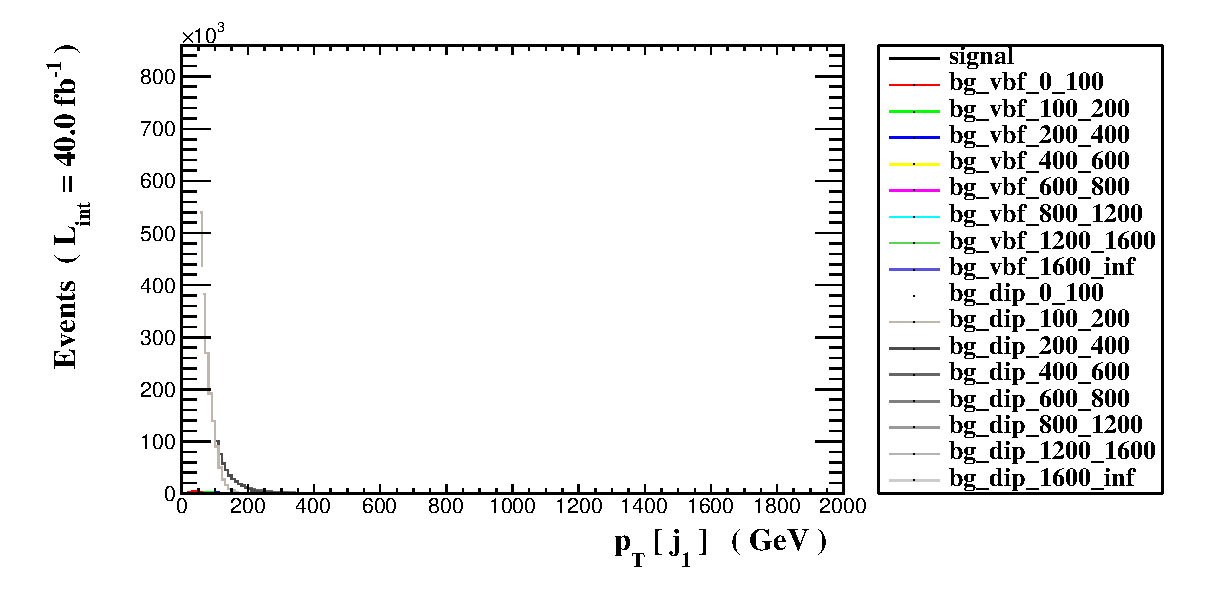
\includegraphics[scale=0.45]{selection_0.eps}\\
\caption{   }
  \end{center}
\end{figure}
      \newpage
\subsection{ Histogram 2}

\textbf{* Plot: ETA ( jets[1] ) }\\
   \begin{table}[H]
  \begin{center}
    \begin{tabular}{|m{23.0mm}|m{23.0mm}|m{18.0mm}|m{19.0mm}|m{19.0mm}|m{19.0mm}|m{19.0mm}|}
      \hline
      {\cellcolor{yellow}         Dataset}& {\cellcolor{yellow}         Integral}& {\cellcolor{yellow}         Entries per event}& {\cellcolor{yellow}         Mean}& {\cellcolor{yellow}         RMS}& {\cellcolor{yellow}         \% underflow}& {\cellcolor{yellow}         \% overflow}\\
      \hline
      {\cellcolor{white}         signal}& {\cellcolor{white}         4094}& {\cellcolor{white}         1.0}& {\cellcolor{white}         -0.0023996}& {\cellcolor{white}         1.616}& {\cellcolor{green}         0.0}& {\cellcolor{green}         0.0}\\
      \hline
      {\cellcolor{white}         bg\_vbf\_0\_100}& {\cellcolor{white}         12150}& {\cellcolor{white}         1.0}& {\cellcolor{white}         0.000371015}& {\cellcolor{white}         2.059}& {\cellcolor{green}         0.0}& {\cellcolor{green}         0.0}\\
      \hline
      {\cellcolor{white}         bg\_vbf\_100\_200}& {\cellcolor{white}         9695}& {\cellcolor{white}         1.0}& {\cellcolor{white}         0.00372318}& {\cellcolor{white}         2.194}& {\cellcolor{green}         0.0}& {\cellcolor{green}         0.0}\\
      \hline
      {\cellcolor{white}         bg\_vbf\_200\_400}& {\cellcolor{white}         5413}& {\cellcolor{white}         1.0}& {\cellcolor{white}         0.00194759}& {\cellcolor{white}         1.96}& {\cellcolor{green}         0.0}& {\cellcolor{green}         0.0}\\
      \hline
      {\cellcolor{white}         bg\_vbf\_400\_600}& {\cellcolor{white}         986}& {\cellcolor{white}         1.0}& {\cellcolor{white}         -0.00101336}& {\cellcolor{white}         1.681}& {\cellcolor{green}         0.0}& {\cellcolor{green}         0.0}\\
      \hline
      {\cellcolor{white}         bg\_vbf\_600\_800}& {\cellcolor{white}         252}& {\cellcolor{white}         1.0}& {\cellcolor{white}         0.000528588}& {\cellcolor{white}         1.498}& {\cellcolor{green}         0.0}& {\cellcolor{green}         0.0}\\
      \hline
      {\cellcolor{white}         bg\_vbf\_800\_1200}& {\cellcolor{white}         114}& {\cellcolor{white}         1.0}& {\cellcolor{white}         -0.00311756}& {\cellcolor{white}         1.329}& {\cellcolor{green}         0.0}& {\cellcolor{green}         0.0}\\
      \hline
      {\cellcolor{white}         bg\_vbf\_1200\_1600}& {\cellcolor{white}         20.6}& {\cellcolor{white}         1.0}& {\cellcolor{white}         -0.000172131}& {\cellcolor{white}         1.134}& {\cellcolor{green}         0.0}& {\cellcolor{green}         0.0}\\
      \hline
      {\cellcolor{white}         bg\_vbf\_1600\_inf}& {\cellcolor{white}         7.66}& {\cellcolor{white}         1.0}& {\cellcolor{white}         0.00127081}& {\cellcolor{white}         0.9541}& {\cellcolor{green}         0.0}& {\cellcolor{green}         0.0}\\
      \hline
      {\cellcolor{white}         bg\_dip\_0\_100}& {\cellcolor{white}         2710844}& {\cellcolor{white}         1.0}& {\cellcolor{white}         -0.000628973}& {\cellcolor{white}         1.791}& {\cellcolor{green}         0.0}& {\cellcolor{green}         0.0}\\
      \hline
      {\cellcolor{white}         bg\_dip\_100\_200}& {\cellcolor{white}         1095361}& {\cellcolor{white}         1.0}& {\cellcolor{white}         0.00112025}& {\cellcolor{white}         1.645}& {\cellcolor{green}         0.0}& {\cellcolor{green}         0.0}\\
      \hline
      {\cellcolor{white}         bg\_dip\_200\_400}& {\cellcolor{white}         239548}& {\cellcolor{white}         1.0}& {\cellcolor{white}         -0.000638999}& {\cellcolor{white}         1.463}& {\cellcolor{green}         0.0}& {\cellcolor{green}         0.0}\\
      \hline
      {\cellcolor{white}         bg\_dip\_400\_600}& {\cellcolor{white}         28798}& {\cellcolor{white}         1.0}& {\cellcolor{white}         -0.0017681}& {\cellcolor{white}         1.278}& {\cellcolor{green}         0.0}& {\cellcolor{green}         0.0}\\
      \hline
      {\cellcolor{white}         bg\_dip\_600\_800}& {\cellcolor{white}         6674}& {\cellcolor{white}         1.0}& {\cellcolor{white}         -0.00486777}& {\cellcolor{white}         1.156}& {\cellcolor{green}         0.0}& {\cellcolor{green}         0.0}\\
      \hline
      {\cellcolor{white}         bg\_dip\_800\_1200}& {\cellcolor{white}         2942}& {\cellcolor{white}         1.0}& {\cellcolor{white}         0.00137964}& {\cellcolor{white}         1.052}& {\cellcolor{green}         0.0}& {\cellcolor{green}         0.0}\\
      \hline
      {\cellcolor{white}         bg\_dip\_1200\_1600}& {\cellcolor{white}         513}& {\cellcolor{white}         1.0}& {\cellcolor{white}         -0.00486293}& {\cellcolor{white}         0.9226}& {\cellcolor{green}         0.0}& {\cellcolor{green}         0.0}\\
      \hline
      {\cellcolor{white}         bg\_dip\_1600\_inf}& {\cellcolor{white}         187}& {\cellcolor{white}         1.0}& {\cellcolor{white}         -0.0010731}& {\cellcolor{white}         0.8}& {\cellcolor{green}         0.0}& {\cellcolor{green}         0.0}\\
\hline
    \end{tabular}
  \end{center}
\end{table}

\begin{figure}[H]
  \begin{center}
    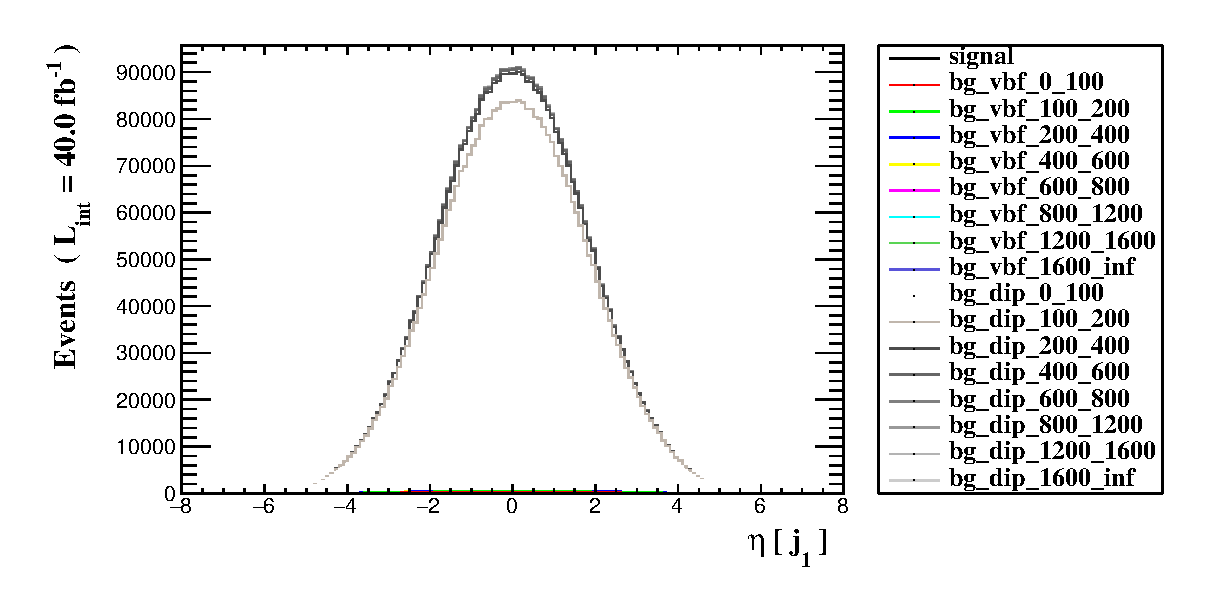
\includegraphics[scale=0.45]{selection_1.eps}\\
\caption{   }
  \end{center}
\end{figure}
      \newpage
\subsection{ Histogram 3}

\textbf{* Plot: PHI ( jets[1] ) }\\
   \begin{table}[H]
  \begin{center}
    \begin{tabular}{|m{23.0mm}|m{23.0mm}|m{18.0mm}|m{19.0mm}|m{19.0mm}|m{19.0mm}|m{19.0mm}|}
      \hline
      {\cellcolor{yellow}         Dataset}& {\cellcolor{yellow}         Integral}& {\cellcolor{yellow}         Entries per event}& {\cellcolor{yellow}         Mean}& {\cellcolor{yellow}         RMS}& {\cellcolor{yellow}         \% underflow}& {\cellcolor{yellow}         \% overflow}\\
      \hline
      {\cellcolor{white}         signal}& {\cellcolor{white}         4094}& {\cellcolor{white}         1.0}& {\cellcolor{white}         0.00102738}& {\cellcolor{white}         1.813}& {\cellcolor{green}         0.0}& {\cellcolor{green}         0.0}\\
      \hline
      {\cellcolor{white}         bg\_vbf\_0\_100}& {\cellcolor{white}         12150}& {\cellcolor{white}         1.0}& {\cellcolor{white}         0.00412621}& {\cellcolor{white}         1.813}& {\cellcolor{green}         0.0}& {\cellcolor{green}         0.0}\\
      \hline
      {\cellcolor{white}         bg\_vbf\_100\_200}& {\cellcolor{white}         9695}& {\cellcolor{white}         1.0}& {\cellcolor{white}         -0.00114327}& {\cellcolor{white}         1.814}& {\cellcolor{green}         0.0}& {\cellcolor{green}         0.0}\\
      \hline
      {\cellcolor{white}         bg\_vbf\_200\_400}& {\cellcolor{white}         5413}& {\cellcolor{white}         1.0}& {\cellcolor{white}         0.00195755}& {\cellcolor{white}         1.814}& {\cellcolor{green}         0.0}& {\cellcolor{green}         0.0}\\
      \hline
      {\cellcolor{white}         bg\_vbf\_400\_600}& {\cellcolor{white}         986}& {\cellcolor{white}         1.0}& {\cellcolor{white}         -0.00347712}& {\cellcolor{white}         1.813}& {\cellcolor{green}         0.0}& {\cellcolor{green}         0.0}\\
      \hline
      {\cellcolor{white}         bg\_vbf\_600\_800}& {\cellcolor{white}         252}& {\cellcolor{white}         1.0}& {\cellcolor{white}         -0.000970243}& {\cellcolor{white}         1.813}& {\cellcolor{green}         0.0}& {\cellcolor{green}         0.0}\\
      \hline
      {\cellcolor{white}         bg\_vbf\_800\_1200}& {\cellcolor{white}         114}& {\cellcolor{white}         1.0}& {\cellcolor{white}         -0.00348235}& {\cellcolor{white}         1.813}& {\cellcolor{green}         0.0}& {\cellcolor{green}         0.0}\\
      \hline
      {\cellcolor{white}         bg\_vbf\_1200\_1600}& {\cellcolor{white}         20.6}& {\cellcolor{white}         1.0}& {\cellcolor{white}         0.00205456}& {\cellcolor{white}         1.813}& {\cellcolor{green}         0.0}& {\cellcolor{green}         0.0}\\
      \hline
      {\cellcolor{white}         bg\_vbf\_1600\_inf}& {\cellcolor{white}         7.66}& {\cellcolor{white}         1.0}& {\cellcolor{white}         0.00218185}& {\cellcolor{white}         1.813}& {\cellcolor{green}         0.0}& {\cellcolor{green}         0.0}\\
      \hline
      {\cellcolor{white}         bg\_dip\_0\_100}& {\cellcolor{white}         2710844}& {\cellcolor{white}         1.0}& {\cellcolor{white}         0.000565782}& {\cellcolor{white}         1.815}& {\cellcolor{green}         0.0}& {\cellcolor{green}         0.0}\\
      \hline
      {\cellcolor{white}         bg\_dip\_100\_200}& {\cellcolor{white}         1095361}& {\cellcolor{white}         1.0}& {\cellcolor{white}         0.000302315}& {\cellcolor{white}         1.815}& {\cellcolor{green}         0.0}& {\cellcolor{green}         0.0}\\
      \hline
      {\cellcolor{white}         bg\_dip\_200\_400}& {\cellcolor{white}         239548}& {\cellcolor{white}         1.0}& {\cellcolor{white}         -0.00160784}& {\cellcolor{white}         1.813}& {\cellcolor{green}         0.0}& {\cellcolor{green}         0.0}\\
      \hline
      {\cellcolor{white}         bg\_dip\_400\_600}& {\cellcolor{white}         28798}& {\cellcolor{white}         1.0}& {\cellcolor{white}         -0.0021849}& {\cellcolor{white}         1.813}& {\cellcolor{green}         0.0}& {\cellcolor{green}         0.0}\\
      \hline
      {\cellcolor{white}         bg\_dip\_600\_800}& {\cellcolor{white}         6674}& {\cellcolor{white}         1.0}& {\cellcolor{white}         0.00111123}& {\cellcolor{white}         1.814}& {\cellcolor{green}         0.0}& {\cellcolor{green}         0.0}\\
      \hline
      {\cellcolor{white}         bg\_dip\_800\_1200}& {\cellcolor{white}         2942}& {\cellcolor{white}         1.0}& {\cellcolor{white}         0.000382954}& {\cellcolor{white}         1.814}& {\cellcolor{green}         0.0}& {\cellcolor{green}         0.0}\\
      \hline
      {\cellcolor{white}         bg\_dip\_1200\_1600}& {\cellcolor{white}         513}& {\cellcolor{white}         1.0}& {\cellcolor{white}         9.82053e-05}& {\cellcolor{white}         1.814}& {\cellcolor{green}         0.0}& {\cellcolor{green}         0.0}\\
      \hline
      {\cellcolor{white}         bg\_dip\_1600\_inf}& {\cellcolor{white}         187}& {\cellcolor{white}         1.0}& {\cellcolor{white}         0.00144174}& {\cellcolor{white}         1.814}& {\cellcolor{green}         0.0}& {\cellcolor{green}         0.0}\\
\hline
    \end{tabular}
  \end{center}
\end{table}

\begin{figure}[H]
  \begin{center}
    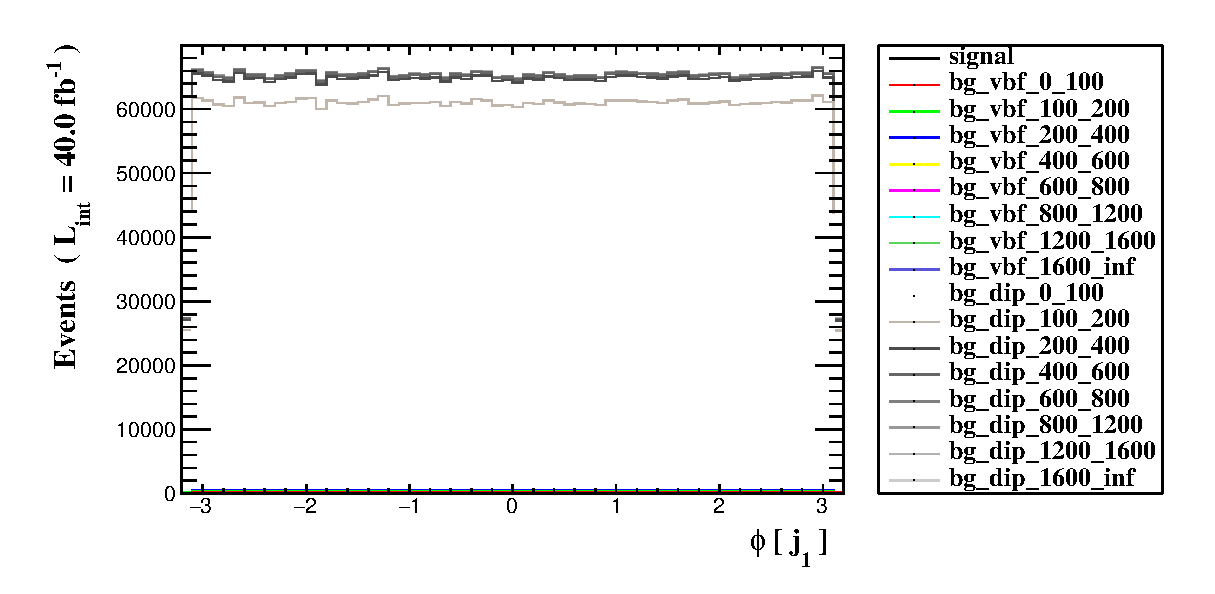
\includegraphics[scale=0.45]{selection_2.eps}\\
\caption{   }
  \end{center}
\end{figure}
      \newpage
\subsection{ Histogram 4}

\textbf{* Plot: PT ( jets[2] ) }\\
   \begin{table}[H]
  \begin{center}
    \begin{tabular}{|m{23.0mm}|m{23.0mm}|m{18.0mm}|m{19.0mm}|m{19.0mm}|m{19.0mm}|m{19.0mm}|}
      \hline
      {\cellcolor{yellow}         Dataset}& {\cellcolor{yellow}         Integral}& {\cellcolor{yellow}         Entries per event}& {\cellcolor{yellow}         Mean}& {\cellcolor{yellow}         RMS}& {\cellcolor{yellow}         \% underflow}& {\cellcolor{yellow}         \% overflow}\\
      \hline
      {\cellcolor{white}         signal}& {\cellcolor{white}         4094}& {\cellcolor{white}         1.0}& {\cellcolor{white}         161.87}& {\cellcolor{white}         136.0}& {\cellcolor{green}         0.0}& {\cellcolor{green}         0.0446}\\
      \hline
      {\cellcolor{white}         bg\_vbf\_0\_100}& {\cellcolor{white}         12150}& {\cellcolor{white}         1.0}& {\cellcolor{white}         29.7897}& {\cellcolor{white}         6.782}& {\cellcolor{green}         0.0}& {\cellcolor{green}         0.0}\\
      \hline
      {\cellcolor{white}         bg\_vbf\_100\_200}& {\cellcolor{white}         9695}& {\cellcolor{white}         1.0}& {\cellcolor{white}         55.7792}& {\cellcolor{white}         17.23}& {\cellcolor{green}         0.0}& {\cellcolor{green}         0.0}\\
      \hline
      {\cellcolor{white}         bg\_vbf\_200\_400}& {\cellcolor{white}         5413}& {\cellcolor{white}         1.0}& {\cellcolor{white}         111.095}& {\cellcolor{white}         32.99}& {\cellcolor{green}         0.0}& {\cellcolor{green}         0.0}\\
      \hline
      {\cellcolor{white}         bg\_vbf\_400\_600}& {\cellcolor{white}         986}& {\cellcolor{white}         1.0}& {\cellcolor{white}         201.201}& {\cellcolor{white}         47.92}& {\cellcolor{green}         0.0}& {\cellcolor{green}         0.0}\\
      \hline
      {\cellcolor{white}         bg\_vbf\_600\_800}& {\cellcolor{white}         252}& {\cellcolor{white}         1.0}& {\cellcolor{white}         293.807}& {\cellcolor{white}         62.95}& {\cellcolor{green}         0.0}& {\cellcolor{green}         0.0}\\
      \hline
      {\cellcolor{white}         bg\_vbf\_800\_1200}& {\cellcolor{white}         114}& {\cellcolor{white}         1.0}& {\cellcolor{white}         415.011}& {\cellcolor{white}         90.61}& {\cellcolor{green}         0.0}& {\cellcolor{green}         0.0}\\
      \hline
      {\cellcolor{white}         bg\_vbf\_1200\_1600}& {\cellcolor{white}         20.6}& {\cellcolor{white}         1.0}& {\cellcolor{white}         613.828}& {\cellcolor{white}         108.5}& {\cellcolor{green}         0.0}& {\cellcolor{green}         0.0}\\
      \hline
      {\cellcolor{white}         bg\_vbf\_1600\_inf}& {\cellcolor{white}         7.66}& {\cellcolor{white}         1.0}& {\cellcolor{white}         917.972}& {\cellcolor{white}         221.8}& {\cellcolor{red}         0.0}& {\cellcolor{red}         25.12}\\
      \hline
      {\cellcolor{white}         bg\_dip\_0\_100}& {\cellcolor{white}         2710844}& {\cellcolor{white}         1.0}& {\cellcolor{white}         27.8531}& {\cellcolor{white}         6.44}& {\cellcolor{green}         0.0}& {\cellcolor{green}         0.0}\\
      \hline
      {\cellcolor{white}         bg\_dip\_100\_200}& {\cellcolor{white}         1095361}& {\cellcolor{white}         1.0}& {\cellcolor{white}         51.3191}& {\cellcolor{white}         16.24}& {\cellcolor{green}         0.0}& {\cellcolor{green}         0.0}\\
      \hline
      {\cellcolor{white}         bg\_dip\_200\_400}& {\cellcolor{white}         239548}& {\cellcolor{white}         1.0}& {\cellcolor{white}         105.003}& {\cellcolor{white}         34.49}& {\cellcolor{green}         0.0}& {\cellcolor{green}         0.0}\\
      \hline
      {\cellcolor{white}         bg\_dip\_400\_600}& {\cellcolor{white}         28798}& {\cellcolor{white}         1.0}& {\cellcolor{white}         200.18}& {\cellcolor{white}         52.16}& {\cellcolor{green}         0.0}& {\cellcolor{green}         0.0}\\
      \hline
      {\cellcolor{white}         bg\_dip\_600\_800}& {\cellcolor{white}         6674}& {\cellcolor{white}         1.0}& {\cellcolor{white}         296.396}& {\cellcolor{white}         65.67}& {\cellcolor{green}         0.0}& {\cellcolor{green}         0.0}\\
      \hline
      {\cellcolor{white}         bg\_dip\_800\_1200}& {\cellcolor{white}         2942}& {\cellcolor{white}         1.0}& {\cellcolor{white}         421.324}& {\cellcolor{white}         89.31}& {\cellcolor{green}         0.0}& {\cellcolor{green}         0.0}\\
      \hline
      {\cellcolor{white}         bg\_dip\_1200\_1600}& {\cellcolor{white}         513}& {\cellcolor{white}         1.0}& {\cellcolor{white}         623.411}& {\cellcolor{white}         99.84}& {\cellcolor{green}         0.0}& {\cellcolor{green}         0.0}\\
      \hline
      {\cellcolor{white}         bg\_dip\_1600\_inf}& {\cellcolor{white}         187}& {\cellcolor{white}         1.0}& {\cellcolor{white}         926.288}& {\cellcolor{white}         210.5}& {\cellcolor{red}         0.0}& {\cellcolor{red}         25.44}\\
\hline
    \end{tabular}
  \end{center}
\end{table}

\begin{figure}[H]
  \begin{center}
    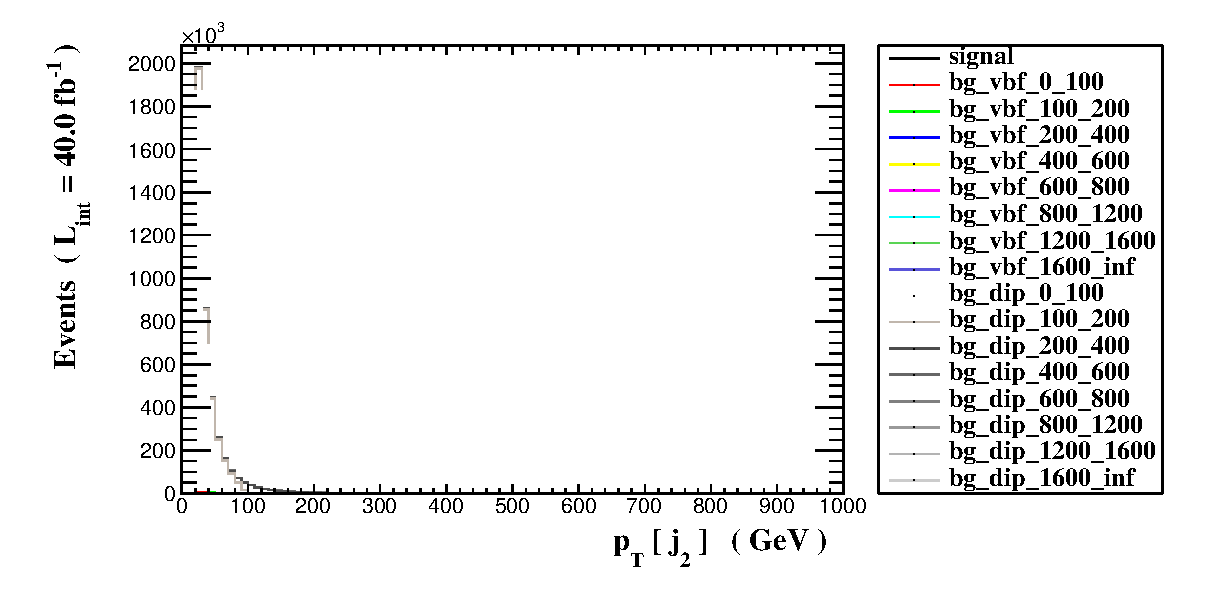
\includegraphics[scale=0.45]{selection_3.eps}\\
\caption{   }
  \end{center}
\end{figure}
      \newpage
\subsection{ Histogram 5}

\textbf{* Plot: ETA ( jets[2] ) }\\
   \begin{table}[H]
  \begin{center}
    \begin{tabular}{|m{23.0mm}|m{23.0mm}|m{18.0mm}|m{19.0mm}|m{19.0mm}|m{19.0mm}|m{19.0mm}|}
      \hline
      {\cellcolor{yellow}         Dataset}& {\cellcolor{yellow}         Integral}& {\cellcolor{yellow}         Entries per event}& {\cellcolor{yellow}         Mean}& {\cellcolor{yellow}         RMS}& {\cellcolor{yellow}         \% underflow}& {\cellcolor{yellow}         \% overflow}\\
      \hline
      {\cellcolor{white}         signal}& {\cellcolor{white}         4094}& {\cellcolor{white}         1.0}& {\cellcolor{white}         0.00500696}& {\cellcolor{white}         2.329}& {\cellcolor{green}         0.0}& {\cellcolor{green}         0.0}\\
      \hline
      {\cellcolor{white}         bg\_vbf\_0\_100}& {\cellcolor{white}         12150}& {\cellcolor{white}         1.0}& {\cellcolor{white}         -0.0012127}& {\cellcolor{white}         2.073}& {\cellcolor{green}         0.0}& {\cellcolor{green}         0.0}\\
      \hline
      {\cellcolor{white}         bg\_vbf\_100\_200}& {\cellcolor{white}         9695}& {\cellcolor{white}         1.0}& {\cellcolor{white}         -0.00624445}& {\cellcolor{white}         2.309}& {\cellcolor{green}         0.0}& {\cellcolor{green}         0.0}\\
      \hline
      {\cellcolor{white}         bg\_vbf\_200\_400}& {\cellcolor{white}         5413}& {\cellcolor{white}         1.0}& {\cellcolor{white}         0.00023751}& {\cellcolor{white}         2.126}& {\cellcolor{green}         0.0}& {\cellcolor{green}         0.0}\\
      \hline
      {\cellcolor{white}         bg\_vbf\_400\_600}& {\cellcolor{white}         986}& {\cellcolor{white}         1.0}& {\cellcolor{white}         -0.000763309}& {\cellcolor{white}         1.861}& {\cellcolor{green}         0.0}& {\cellcolor{green}         0.0}\\
      \hline
      {\cellcolor{white}         bg\_vbf\_600\_800}& {\cellcolor{white}         252}& {\cellcolor{white}         1.0}& {\cellcolor{white}         -0.00167246}& {\cellcolor{white}         1.666}& {\cellcolor{green}         0.0}& {\cellcolor{green}         0.0}\\
      \hline
      {\cellcolor{white}         bg\_vbf\_800\_1200}& {\cellcolor{white}         114}& {\cellcolor{white}         1.0}& {\cellcolor{white}         -0.000468537}& {\cellcolor{white}         1.473}& {\cellcolor{green}         0.0}& {\cellcolor{green}         0.0}\\
      \hline
      {\cellcolor{white}         bg\_vbf\_1200\_1600}& {\cellcolor{white}         20.6}& {\cellcolor{white}         1.0}& {\cellcolor{white}         0.000592645}& {\cellcolor{white}         1.238}& {\cellcolor{green}         0.0}& {\cellcolor{green}         0.0}\\
      \hline
      {\cellcolor{white}         bg\_vbf\_1600\_inf}& {\cellcolor{white}         7.66}& {\cellcolor{white}         1.0}& {\cellcolor{white}         -0.00207042}& {\cellcolor{white}         1.017}& {\cellcolor{green}         0.0}& {\cellcolor{green}         0.0}\\
      \hline
      {\cellcolor{white}         bg\_dip\_0\_100}& {\cellcolor{white}         2710844}& {\cellcolor{white}         1.0}& {\cellcolor{white}         0.00019908}& {\cellcolor{white}         1.748}& {\cellcolor{green}         0.0}& {\cellcolor{green}         0.0}\\
      \hline
      {\cellcolor{white}         bg\_dip\_100\_200}& {\cellcolor{white}         1095361}& {\cellcolor{white}         1.0}& {\cellcolor{white}         -0.00179844}& {\cellcolor{white}         1.594}& {\cellcolor{green}         0.0}& {\cellcolor{green}         0.0}\\
      \hline
      {\cellcolor{white}         bg\_dip\_200\_400}& {\cellcolor{white}         239548}& {\cellcolor{white}         1.0}& {\cellcolor{white}         -0.00217858}& {\cellcolor{white}         1.442}& {\cellcolor{green}         0.0}& {\cellcolor{green}         0.0}\\
      \hline
      {\cellcolor{white}         bg\_dip\_400\_600}& {\cellcolor{white}         28798}& {\cellcolor{white}         1.0}& {\cellcolor{white}         -0.000407628}& {\cellcolor{white}         1.289}& {\cellcolor{green}         0.0}& {\cellcolor{green}         0.0}\\
      \hline
      {\cellcolor{white}         bg\_dip\_600\_800}& {\cellcolor{white}         6674}& {\cellcolor{white}         1.0}& {\cellcolor{white}         -0.000290936}& {\cellcolor{white}         1.181}& {\cellcolor{green}         0.0}& {\cellcolor{green}         0.0}\\
      \hline
      {\cellcolor{white}         bg\_dip\_800\_1200}& {\cellcolor{white}         2942}& {\cellcolor{white}         1.0}& {\cellcolor{white}         0.00123653}& {\cellcolor{white}         1.078}& {\cellcolor{green}         0.0}& {\cellcolor{green}         0.0}\\
      \hline
      {\cellcolor{white}         bg\_dip\_1200\_1600}& {\cellcolor{white}         513}& {\cellcolor{white}         1.0}& {\cellcolor{white}         -0.000424243}& {\cellcolor{white}         0.9457}& {\cellcolor{green}         0.0}& {\cellcolor{green}         0.0}\\
      \hline
      {\cellcolor{white}         bg\_dip\_1600\_inf}& {\cellcolor{white}         187}& {\cellcolor{white}         1.0}& {\cellcolor{white}         0.000907795}& {\cellcolor{white}         0.8179}& {\cellcolor{green}         0.0}& {\cellcolor{green}         0.0}\\
\hline
    \end{tabular}
  \end{center}
\end{table}

\begin{figure}[H]
  \begin{center}
    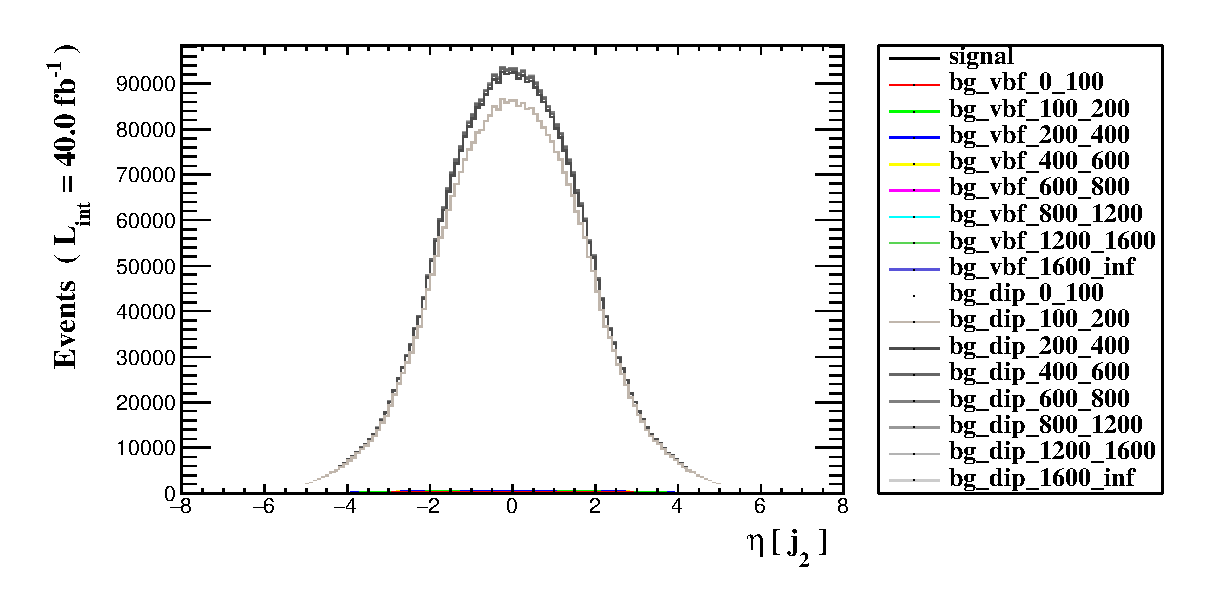
\includegraphics[scale=0.45]{selection_4.eps}\\
\caption{   }
  \end{center}
\end{figure}
      \newpage
\subsection{ Histogram 6}

\textbf{* Plot: PHI ( jets[2] ) }\\
   \begin{table}[H]
  \begin{center}
    \begin{tabular}{|m{23.0mm}|m{23.0mm}|m{18.0mm}|m{19.0mm}|m{19.0mm}|m{19.0mm}|m{19.0mm}|}
      \hline
      {\cellcolor{yellow}         Dataset}& {\cellcolor{yellow}         Integral}& {\cellcolor{yellow}         Entries per event}& {\cellcolor{yellow}         Mean}& {\cellcolor{yellow}         RMS}& {\cellcolor{yellow}         \% underflow}& {\cellcolor{yellow}         \% overflow}\\
      \hline
      {\cellcolor{white}         signal}& {\cellcolor{white}         4094}& {\cellcolor{white}         1.0}& {\cellcolor{white}         -0.00274458}& {\cellcolor{white}         1.814}& {\cellcolor{green}         0.0}& {\cellcolor{green}         0.0}\\
      \hline
      {\cellcolor{white}         bg\_vbf\_0\_100}& {\cellcolor{white}         12150}& {\cellcolor{white}         1.0}& {\cellcolor{white}         -0.000390721}& {\cellcolor{white}         1.815}& {\cellcolor{green}         0.0}& {\cellcolor{green}         0.0}\\
      \hline
      {\cellcolor{white}         bg\_vbf\_100\_200}& {\cellcolor{white}         9695}& {\cellcolor{white}         1.0}& {\cellcolor{white}         -0.000748165}& {\cellcolor{white}         1.814}& {\cellcolor{green}         0.0}& {\cellcolor{green}         0.0}\\
      \hline
      {\cellcolor{white}         bg\_vbf\_200\_400}& {\cellcolor{white}         5413}& {\cellcolor{white}         1.0}& {\cellcolor{white}         -0.00148399}& {\cellcolor{white}         1.814}& {\cellcolor{green}         0.0}& {\cellcolor{green}         0.0}\\
      \hline
      {\cellcolor{white}         bg\_vbf\_400\_600}& {\cellcolor{white}         986}& {\cellcolor{white}         1.0}& {\cellcolor{white}         0.00309107}& {\cellcolor{white}         1.814}& {\cellcolor{green}         0.0}& {\cellcolor{green}         0.0}\\
      \hline
      {\cellcolor{white}         bg\_vbf\_600\_800}& {\cellcolor{white}         252}& {\cellcolor{white}         1.0}& {\cellcolor{white}         0.000470979}& {\cellcolor{white}         1.815}& {\cellcolor{green}         0.0}& {\cellcolor{green}         0.0}\\
      \hline
      {\cellcolor{white}         bg\_vbf\_800\_1200}& {\cellcolor{white}         114}& {\cellcolor{white}         1.0}& {\cellcolor{white}         0.000124126}& {\cellcolor{white}         1.813}& {\cellcolor{green}         0.0}& {\cellcolor{green}         0.0}\\
      \hline
      {\cellcolor{white}         bg\_vbf\_1200\_1600}& {\cellcolor{white}         20.6}& {\cellcolor{white}         1.0}& {\cellcolor{white}         -0.00342189}& {\cellcolor{white}         1.815}& {\cellcolor{green}         0.0}& {\cellcolor{green}         0.0}\\
      \hline
      {\cellcolor{white}         bg\_vbf\_1600\_inf}& {\cellcolor{white}         7.66}& {\cellcolor{white}         1.0}& {\cellcolor{white}         -0.00282812}& {\cellcolor{white}         1.814}& {\cellcolor{green}         0.0}& {\cellcolor{green}         0.0}\\
      \hline
      {\cellcolor{white}         bg\_dip\_0\_100}& {\cellcolor{white}         2710844}& {\cellcolor{white}         1.0}& {\cellcolor{white}         0.000242632}& {\cellcolor{white}         1.812}& {\cellcolor{green}         0.0}& {\cellcolor{green}         0.0}\\
      \hline
      {\cellcolor{white}         bg\_dip\_100\_200}& {\cellcolor{white}         1095361}& {\cellcolor{white}         1.0}& {\cellcolor{white}         0.000855811}& {\cellcolor{white}         1.814}& {\cellcolor{green}         0.0}& {\cellcolor{green}         0.0}\\
      \hline
      {\cellcolor{white}         bg\_dip\_200\_400}& {\cellcolor{white}         239548}& {\cellcolor{white}         1.0}& {\cellcolor{white}         0.000682802}& {\cellcolor{white}         1.815}& {\cellcolor{green}         0.0}& {\cellcolor{green}         0.0}\\
      \hline
      {\cellcolor{white}         bg\_dip\_400\_600}& {\cellcolor{white}         28798}& {\cellcolor{white}         1.0}& {\cellcolor{white}         9.86323e-05}& {\cellcolor{white}         1.814}& {\cellcolor{green}         0.0}& {\cellcolor{green}         0.0}\\
      \hline
      {\cellcolor{white}         bg\_dip\_600\_800}& {\cellcolor{white}         6674}& {\cellcolor{white}         1.0}& {\cellcolor{white}         -0.00254972}& {\cellcolor{white}         1.815}& {\cellcolor{green}         0.0}& {\cellcolor{green}         0.0}\\
      \hline
      {\cellcolor{white}         bg\_dip\_800\_1200}& {\cellcolor{white}         2942}& {\cellcolor{white}         1.0}& {\cellcolor{white}         -0.000758074}& {\cellcolor{white}         1.813}& {\cellcolor{green}         0.0}& {\cellcolor{green}         0.0}\\
      \hline
      {\cellcolor{white}         bg\_dip\_1200\_1600}& {\cellcolor{white}         513}& {\cellcolor{white}         1.0}& {\cellcolor{white}         -0.00202378}& {\cellcolor{white}         1.813}& {\cellcolor{green}         0.0}& {\cellcolor{green}         0.0}\\
      \hline
      {\cellcolor{white}         bg\_dip\_1600\_inf}& {\cellcolor{white}         187}& {\cellcolor{white}         1.0}& {\cellcolor{white}         0.00235585}& {\cellcolor{white}         1.814}& {\cellcolor{green}         0.0}& {\cellcolor{green}         0.0}\\
\hline
    \end{tabular}
  \end{center}
\end{table}

\begin{figure}[H]
  \begin{center}
    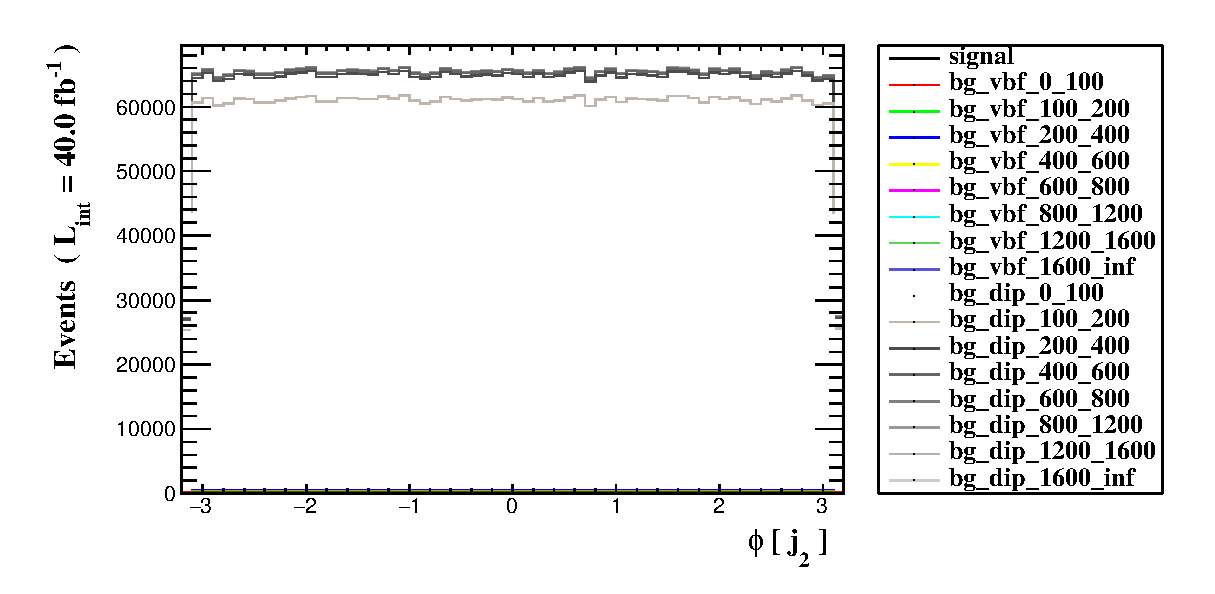
\includegraphics[scale=0.45]{selection_5.eps}\\
\caption{   }
  \end{center}
\end{figure}
      \newpage
\subsection{ Histogram 7}

\textbf{* Plot: DELTAR ( jets[1] , jets[2] ) }\\
   \begin{table}[H]
  \begin{center}
    \begin{tabular}{|m{23.0mm}|m{23.0mm}|m{18.0mm}|m{19.0mm}|m{19.0mm}|m{19.0mm}|m{19.0mm}|}
      \hline
      {\cellcolor{yellow}         Dataset}& {\cellcolor{yellow}         Integral}& {\cellcolor{yellow}         Entries per event}& {\cellcolor{yellow}         Mean}& {\cellcolor{yellow}         RMS}& {\cellcolor{yellow}         \% underflow}& {\cellcolor{yellow}         \% overflow}\\
      \hline
      {\cellcolor{white}         signal}& {\cellcolor{white}         4094}& {\cellcolor{white}         1.0}& {\cellcolor{white}         4.02835}& {\cellcolor{white}         1.056}& {\cellcolor{green}         0.0}& {\cellcolor{green}         0.0}\\
      \hline
      {\cellcolor{white}         bg\_vbf\_0\_100}& {\cellcolor{white}         12150}& {\cellcolor{white}         1.0}& {\cellcolor{white}         3.6437}& {\cellcolor{white}         1.351}& {\cellcolor{green}         0.0}& {\cellcolor{green}         0.0}\\
      \hline
      {\cellcolor{white}         bg\_vbf\_100\_200}& {\cellcolor{white}         9695}& {\cellcolor{white}         1.0}& {\cellcolor{white}         4.43942}& {\cellcolor{white}         1.431}& {\cellcolor{green}         0.0}& {\cellcolor{green}         0.0}\\
      \hline
      {\cellcolor{white}         bg\_vbf\_200\_400}& {\cellcolor{white}         5413}& {\cellcolor{white}         1.0}& {\cellcolor{white}         4.36935}& {\cellcolor{white}         1.146}& {\cellcolor{green}         0.0}& {\cellcolor{green}         0.0}\\
      \hline
      {\cellcolor{white}         bg\_vbf\_400\_600}& {\cellcolor{white}         986}& {\cellcolor{white}         1.0}& {\cellcolor{white}         4.1046}& {\cellcolor{white}         0.9149}& {\cellcolor{green}         0.0}& {\cellcolor{green}         0.0}\\
      \hline
      {\cellcolor{white}         bg\_vbf\_600\_800}& {\cellcolor{white}         252}& {\cellcolor{white}         1.0}& {\cellcolor{white}         3.92394}& {\cellcolor{white}         0.7774}& {\cellcolor{green}         0.0}& {\cellcolor{green}         0.0}\\
      \hline
      {\cellcolor{white}         bg\_vbf\_800\_1200}& {\cellcolor{white}         114}& {\cellcolor{white}         1.0}& {\cellcolor{white}         3.75769}& {\cellcolor{white}         0.6598}& {\cellcolor{green}         0.0}& {\cellcolor{green}         0.0}\\
      \hline
      {\cellcolor{white}         bg\_vbf\_1200\_1600}& {\cellcolor{white}         20.6}& {\cellcolor{white}         1.0}& {\cellcolor{white}         3.58471}& {\cellcolor{white}         0.5261}& {\cellcolor{green}         0.0}& {\cellcolor{green}         0.0}\\
      \hline
      {\cellcolor{white}         bg\_vbf\_1600\_inf}& {\cellcolor{white}         7.66}& {\cellcolor{white}         1.0}& {\cellcolor{white}         3.44779}& {\cellcolor{white}         0.4108}& {\cellcolor{green}         0.0}& {\cellcolor{green}         0.0}\\
      \hline
      {\cellcolor{white}         bg\_dip\_0\_100}& {\cellcolor{white}         2710844}& {\cellcolor{white}         1.0}& {\cellcolor{white}         3.17806}& {\cellcolor{white}         0.938}& {\cellcolor{green}         0.0}& {\cellcolor{green}         0.0}\\
      \hline
      {\cellcolor{white}         bg\_dip\_100\_200}& {\cellcolor{white}         1095361}& {\cellcolor{white}         1.0}& {\cellcolor{white}         3.22987}& {\cellcolor{white}         0.8214}& {\cellcolor{green}         0.0}& {\cellcolor{green}         0.0}\\
      \hline
      {\cellcolor{white}         bg\_dip\_200\_400}& {\cellcolor{white}         239548}& {\cellcolor{white}         1.0}& {\cellcolor{white}         3.25054}& {\cellcolor{white}         0.7204}& {\cellcolor{green}         0.0}& {\cellcolor{green}         0.0}\\
      \hline
      {\cellcolor{white}         bg\_dip\_400\_600}& {\cellcolor{white}         28798}& {\cellcolor{white}         1.0}& {\cellcolor{white}         3.27012}& {\cellcolor{white}         0.6166}& {\cellcolor{green}         0.0}& {\cellcolor{green}         0.0}\\
      \hline
      {\cellcolor{white}         bg\_dip\_600\_800}& {\cellcolor{white}         6674}& {\cellcolor{white}         1.0}& {\cellcolor{white}         3.27863}& {\cellcolor{white}         0.5424}& {\cellcolor{green}         0.0}& {\cellcolor{green}         0.0}\\
      \hline
      {\cellcolor{white}         bg\_dip\_800\_1200}& {\cellcolor{white}         2942}& {\cellcolor{white}         1.0}& {\cellcolor{white}         3.28404}& {\cellcolor{white}         0.4723}& {\cellcolor{green}         0.0}& {\cellcolor{green}         0.0}\\
      \hline
      {\cellcolor{white}         bg\_dip\_1200\_1600}& {\cellcolor{white}         513}& {\cellcolor{white}         1.0}& {\cellcolor{white}         3.2807}& {\cellcolor{white}         0.3852}& {\cellcolor{green}         0.0}& {\cellcolor{green}         0.0}\\
      \hline
      {\cellcolor{white}         bg\_dip\_1600\_inf}& {\cellcolor{white}         187}& {\cellcolor{white}         1.0}& {\cellcolor{white}         3.26767}& {\cellcolor{white}         0.3024}& {\cellcolor{green}         0.0}& {\cellcolor{green}         0.0}\\
\hline
    \end{tabular}
  \end{center}
\end{table}

\begin{figure}[H]
  \begin{center}
    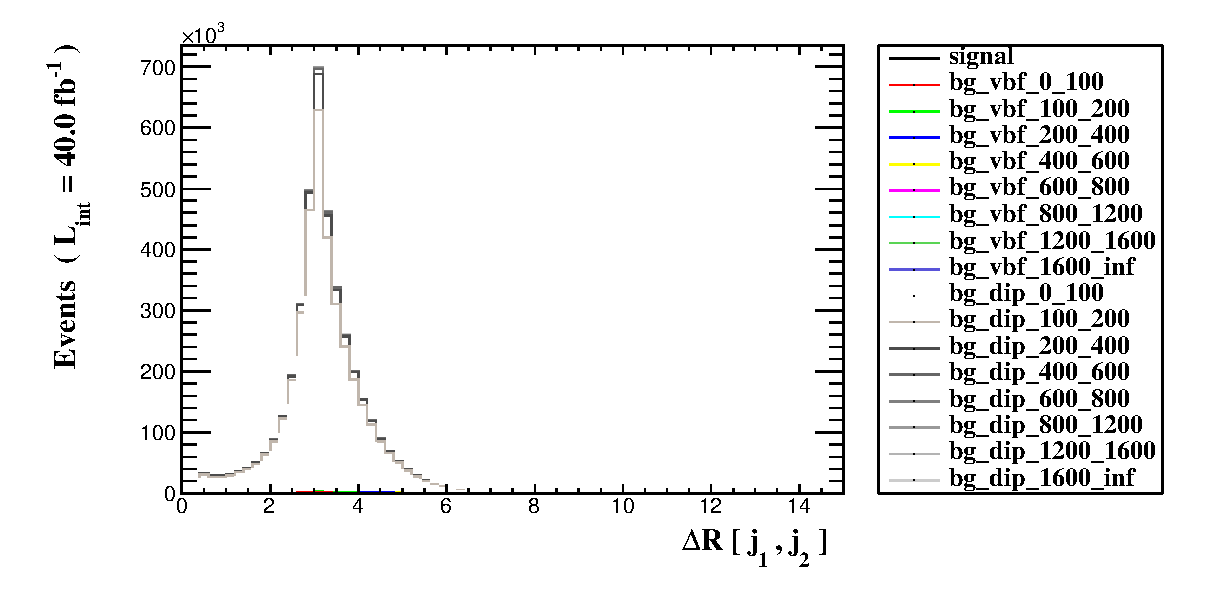
\includegraphics[scale=0.45]{selection_6.eps}\\
\caption{   }
  \end{center}
\end{figure}
      \newpage
\subsection{ Histogram 8}

\textbf{* Plot: M ( jets[1] jets[2] ) }\\
   \begin{table}[H]
  \begin{center}
    \begin{tabular}{|m{23.0mm}|m{23.0mm}|m{18.0mm}|m{19.0mm}|m{19.0mm}|m{19.0mm}|m{19.0mm}|}
      \hline
      {\cellcolor{yellow}         Dataset}& {\cellcolor{yellow}         Integral}& {\cellcolor{yellow}         Entries per event}& {\cellcolor{yellow}         Mean}& {\cellcolor{yellow}         RMS}& {\cellcolor{yellow}         \% underflow}& {\cellcolor{yellow}         \% overflow}\\
      \hline
      {\cellcolor{white}         signal}& {\cellcolor{white}         4094}& {\cellcolor{white}         1.0}& {\cellcolor{white}         1376.2}& {\cellcolor{white}         772.9}& {\cellcolor{green}         0.0}& {\cellcolor{green}         0.0}\\
      \hline
      {\cellcolor{white}         bg\_vbf\_0\_100}& {\cellcolor{white}         12150}& {\cellcolor{white}         1.0}& {\cellcolor{white}         204.768}& {\cellcolor{white}         298.2}& {\cellcolor{green}         0.0}& {\cellcolor{green}         0.0}\\
      \hline
      {\cellcolor{white}         bg\_vbf\_100\_200}& {\cellcolor{white}         9695}& {\cellcolor{white}         1.0}& {\cellcolor{white}         559.274}& {\cellcolor{white}         525.7}& {\cellcolor{green}         0.0}& {\cellcolor{green}         0.0}\\
      \hline
      {\cellcolor{white}         bg\_vbf\_200\_400}& {\cellcolor{white}         5413}& {\cellcolor{white}         1.0}& {\cellcolor{white}         880.56}& {\cellcolor{white}         672.7}& {\cellcolor{green}         0.0}& {\cellcolor{green}         0.0003051}\\
      \hline
      {\cellcolor{white}         bg\_vbf\_400\_600}& {\cellcolor{white}         986}& {\cellcolor{white}         1.0}& {\cellcolor{white}         1208.33}& {\cellcolor{white}         762.5}& {\cellcolor{green}         0.0}& {\cellcolor{green}         0.0006}\\
      \hline
      {\cellcolor{white}         bg\_vbf\_600\_800}& {\cellcolor{white}         252}& {\cellcolor{white}         1.0}& {\cellcolor{white}         1464.21}& {\cellcolor{white}         805.7}& {\cellcolor{green}         0.0}& {\cellcolor{green}         0.0014}\\
      \hline
      {\cellcolor{white}         bg\_vbf\_800\_1200}& {\cellcolor{white}         114}& {\cellcolor{white}         1.0}& {\cellcolor{white}         1732.18}& {\cellcolor{white}         822.2}& {\cellcolor{green}         0.0}& {\cellcolor{green}         0.002495}\\
      \hline
      {\cellcolor{white}         bg\_vbf\_1200\_1600}& {\cellcolor{white}         20.6}& {\cellcolor{white}         1.0}& {\cellcolor{white}         2125.24}& {\cellcolor{white}         815.9}& {\cellcolor{green}         0.0}& {\cellcolor{green}         0.002831}\\
      \hline
      {\cellcolor{white}         bg\_vbf\_1600\_inf}& {\cellcolor{white}         7.66}& {\cellcolor{white}         1.0}& {\cellcolor{white}         2691.74}& {\cellcolor{white}         857.1}& {\cellcolor{green}         0.0}& {\cellcolor{green}         0.01037}\\
      \hline
      {\cellcolor{white}         bg\_dip\_0\_100}& {\cellcolor{white}         2710844}& {\cellcolor{white}         1.0}& {\cellcolor{white}         108.441}& {\cellcolor{white}         80.26}& {\cellcolor{green}         0.0}& {\cellcolor{green}         0.0}\\
      \hline
      {\cellcolor{white}         bg\_dip\_100\_200}& {\cellcolor{white}         1095361}& {\cellcolor{white}         1.0}& {\cellcolor{white}         194.945}& {\cellcolor{white}         125.9}& {\cellcolor{green}         0.0}& {\cellcolor{green}         0.0}\\
      \hline
      {\cellcolor{white}         bg\_dip\_200\_400}& {\cellcolor{white}         239548}& {\cellcolor{white}         1.0}& {\cellcolor{white}         358.574}& {\cellcolor{white}         197.8}& {\cellcolor{green}         0.0}& {\cellcolor{green}         0.0}\\
      \hline
      {\cellcolor{white}         bg\_dip\_400\_600}& {\cellcolor{white}         28798}& {\cellcolor{white}         1.0}& {\cellcolor{white}         622.657}& {\cellcolor{white}         280.2}& {\cellcolor{green}         0.0}& {\cellcolor{green}         0.0}\\
      \hline
      {\cellcolor{white}         bg\_dip\_600\_800}& {\cellcolor{white}         6674}& {\cellcolor{white}         1.0}& {\cellcolor{white}         871.188}& {\cellcolor{white}         339.5}& {\cellcolor{green}         0.0}& {\cellcolor{green}         0.0}\\
      \hline
      {\cellcolor{white}         bg\_dip\_800\_1200}& {\cellcolor{white}         2942}& {\cellcolor{white}         1.0}& {\cellcolor{white}         1177.62}& {\cellcolor{white}         409.7}& {\cellcolor{green}         0.0}& {\cellcolor{green}         0.0}\\
      \hline
      {\cellcolor{white}         bg\_dip\_1200\_1600}& {\cellcolor{white}         513}& {\cellcolor{white}         1.0}& {\cellcolor{white}         1647.72}& {\cellcolor{white}         468.6}& {\cellcolor{green}         0.0}& {\cellcolor{green}         0.0}\\
      \hline
      {\cellcolor{white}         bg\_dip\_1600\_inf}& {\cellcolor{white}         187}& {\cellcolor{white}         1.0}& {\cellcolor{white}         2311.53}& {\cellcolor{white}         635.5}& {\cellcolor{green}         0.0}& {\cellcolor{green}         0.0001923}\\
\hline
    \end{tabular}
  \end{center}
\end{table}

\begin{figure}[H]
  \begin{center}
    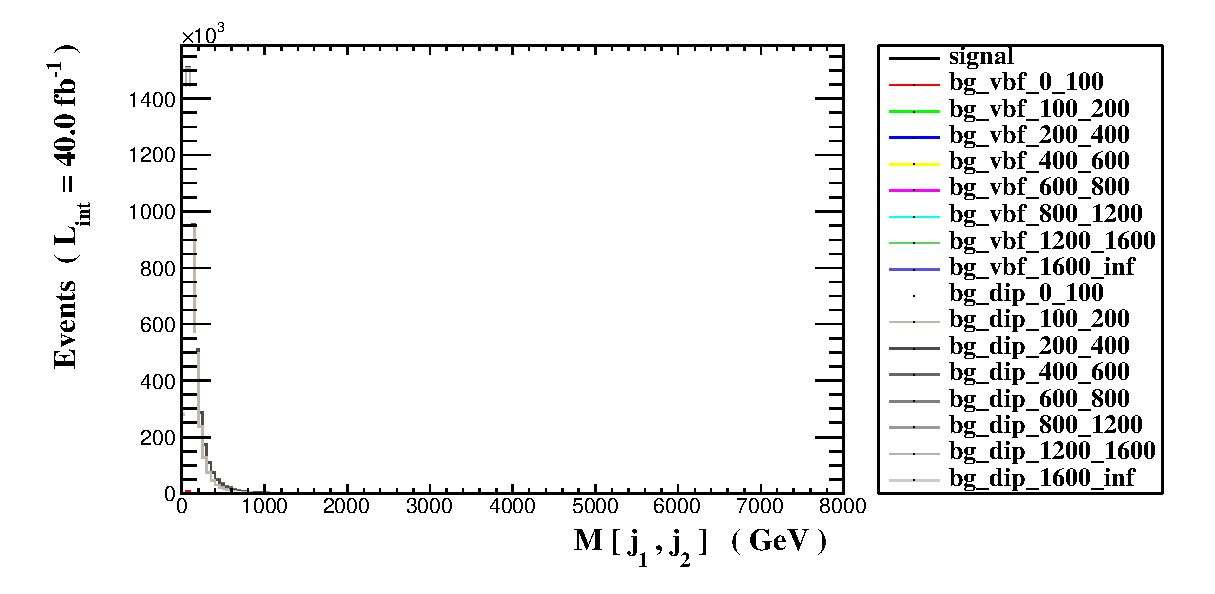
\includegraphics[scale=0.45]{selection_7.eps}\\
\caption{   }
  \end{center}
\end{figure}
      \newpage
\subsection{ Histogram 9}

\textbf{* Plot: sdETA ( jets[1] jets[2] ) }\\
   \begin{table}[H]
  \begin{center}
    \begin{tabular}{|m{23.0mm}|m{23.0mm}|m{18.0mm}|m{19.0mm}|m{19.0mm}|m{19.0mm}|m{19.0mm}|}
      \hline
      {\cellcolor{yellow}         Dataset}& {\cellcolor{yellow}         Integral}& {\cellcolor{yellow}         Entries per event}& {\cellcolor{yellow}         Mean}& {\cellcolor{yellow}         RMS}& {\cellcolor{yellow}         \% underflow}& {\cellcolor{yellow}         \% overflow}\\
      \hline
      {\cellcolor{white}         signal}& {\cellcolor{white}         4094}& {\cellcolor{white}         1.0}& {\cellcolor{white}         -0.00740656}& {\cellcolor{white}         3.704}& {\cellcolor{green}         0.0}& {\cellcolor{green}         0.0}\\
      \hline
      {\cellcolor{white}         bg\_vbf\_0\_100}& {\cellcolor{white}         12150}& {\cellcolor{white}         1.0}& {\cellcolor{white}         0.00158372}& {\cellcolor{white}         2.865}& {\cellcolor{green}         0.0}& {\cellcolor{green}         0.0}\\
      \hline
      {\cellcolor{white}         bg\_vbf\_100\_200}& {\cellcolor{white}         9695}& {\cellcolor{white}         1.0}& {\cellcolor{white}         0.00996763}& {\cellcolor{white}         3.823}& {\cellcolor{green}         0.0}& {\cellcolor{green}         0.0}\\
      \hline
      {\cellcolor{white}         bg\_vbf\_200\_400}& {\cellcolor{white}         5413}& {\cellcolor{white}         1.0}& {\cellcolor{white}         0.00171008}& {\cellcolor{white}         3.551}& {\cellcolor{green}         0.0}& {\cellcolor{green}         0.0}\\
      \hline
      {\cellcolor{white}         bg\_vbf\_400\_600}& {\cellcolor{white}         986}& {\cellcolor{white}         1.0}& {\cellcolor{white}         -0.000250051}& {\cellcolor{white}         3.085}& {\cellcolor{green}         0.0}& {\cellcolor{green}         0.0}\\
      \hline
      {\cellcolor{white}         bg\_vbf\_600\_800}& {\cellcolor{white}         252}& {\cellcolor{white}         1.0}& {\cellcolor{white}         0.00220104}& {\cellcolor{white}         2.753}& {\cellcolor{green}         0.0}& {\cellcolor{green}         0.0}\\
      \hline
      {\cellcolor{white}         bg\_vbf\_800\_1200}& {\cellcolor{white}         114}& {\cellcolor{white}         1.0}& {\cellcolor{white}         -0.00264902}& {\cellcolor{white}         2.428}& {\cellcolor{green}         0.0}& {\cellcolor{green}         0.0}\\
      \hline
      {\cellcolor{white}         bg\_vbf\_1200\_1600}& {\cellcolor{white}         20.6}& {\cellcolor{white}         1.0}& {\cellcolor{white}         -0.000764776}& {\cellcolor{white}         2.046}& {\cellcolor{green}         0.0}& {\cellcolor{green}         0.0}\\
      \hline
      {\cellcolor{white}         bg\_vbf\_1600\_inf}& {\cellcolor{white}         7.66}& {\cellcolor{white}         1.0}& {\cellcolor{white}         0.00334122}& {\cellcolor{white}         1.694}& {\cellcolor{green}         0.0}& {\cellcolor{green}         0.0}\\
      \hline
      {\cellcolor{white}         bg\_dip\_0\_100}& {\cellcolor{white}         2710844}& {\cellcolor{white}         1.0}& {\cellcolor{white}         -0.000828053}& {\cellcolor{white}         2.094}& {\cellcolor{green}         0.0}& {\cellcolor{green}         0.0}\\
      \hline
      {\cellcolor{white}         bg\_dip\_100\_200}& {\cellcolor{white}         1095361}& {\cellcolor{white}         1.0}& {\cellcolor{white}         0.00291869}& {\cellcolor{white}         1.936}& {\cellcolor{green}         0.0}& {\cellcolor{green}         0.0}\\
      \hline
      {\cellcolor{white}         bg\_dip\_200\_400}& {\cellcolor{white}         239548}& {\cellcolor{white}         1.0}& {\cellcolor{white}         0.00153958}& {\cellcolor{white}         1.779}& {\cellcolor{green}         0.0}& {\cellcolor{green}         0.0}\\
      \hline
      {\cellcolor{white}         bg\_dip\_400\_600}& {\cellcolor{white}         28798}& {\cellcolor{white}         1.0}& {\cellcolor{white}         -0.00136047}& {\cellcolor{white}         1.634}& {\cellcolor{green}         0.0}& {\cellcolor{green}         0.0}\\
      \hline
      {\cellcolor{white}         bg\_dip\_600\_800}& {\cellcolor{white}         6674}& {\cellcolor{white}         1.0}& {\cellcolor{white}         -0.00457683}& {\cellcolor{white}         1.538}& {\cellcolor{green}         0.0}& {\cellcolor{green}         0.0}\\
      \hline
      {\cellcolor{white}         bg\_dip\_800\_1200}& {\cellcolor{white}         2942}& {\cellcolor{white}         1.0}& {\cellcolor{white}         0.000143111}& {\cellcolor{white}         1.448}& {\cellcolor{green}         0.0}& {\cellcolor{green}         0.0}\\
      \hline
      {\cellcolor{white}         bg\_dip\_1200\_1600}& {\cellcolor{white}         513}& {\cellcolor{white}         1.0}& {\cellcolor{white}         -0.00443869}& {\cellcolor{white}         1.327}& {\cellcolor{green}         0.0}& {\cellcolor{green}         0.0}\\
      \hline
      {\cellcolor{white}         bg\_dip\_1600\_inf}& {\cellcolor{white}         187}& {\cellcolor{white}         1.0}& {\cellcolor{white}         -0.0019809}& {\cellcolor{white}         1.196}& {\cellcolor{green}         0.0}& {\cellcolor{green}         0.0}\\
\hline
    \end{tabular}
  \end{center}
\end{table}

\begin{figure}[H]
  \begin{center}
    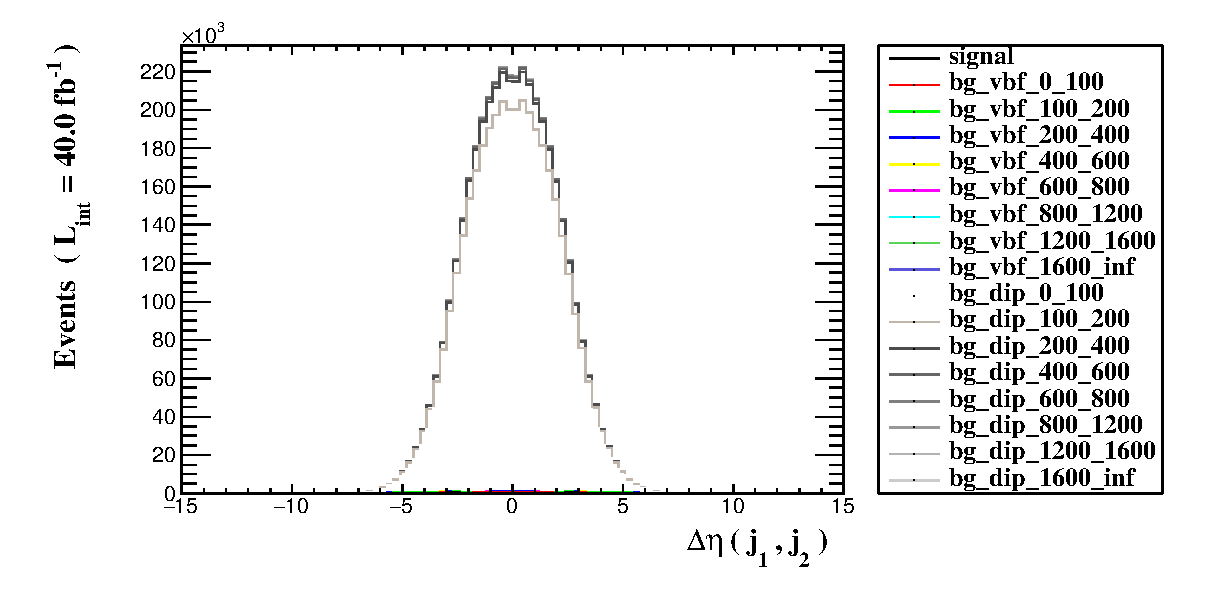
\includegraphics[scale=0.45]{selection_8.eps}\\
\caption{   }
  \end{center}
\end{figure}
      \newpage
\subsection{ Histogram 10}

\textbf{* Plot: M ( a[1] a[2] ) }\\
   \begin{table}[H]
  \begin{center}
    \begin{tabular}{|m{23.0mm}|m{23.0mm}|m{18.0mm}|m{19.0mm}|m{19.0mm}|m{19.0mm}|m{19.0mm}|}
      \hline
      {\cellcolor{yellow}         Dataset}& {\cellcolor{yellow}         Integral}& {\cellcolor{yellow}         Entries per event}& {\cellcolor{yellow}         Mean}& {\cellcolor{yellow}         RMS}& {\cellcolor{yellow}         \% underflow}& {\cellcolor{yellow}         \% overflow}\\
      \hline
      {\cellcolor{white}         signal}& {\cellcolor{white}         4094}& {\cellcolor{white}         1.0}& {\cellcolor{white}         950.206}& {\cellcolor{white}         725.5}& {\cellcolor{green}         0.0}& {\cellcolor{green}         0.3972}\\
      \hline
      {\cellcolor{white}         bg\_vbf\_0\_100}& {\cellcolor{white}         12150}& {\cellcolor{white}         1.0}& {\cellcolor{white}         49.9447}& {\cellcolor{white}         41.51}& {\cellcolor{green}         0.0}& {\cellcolor{green}         0.0}\\
      \hline
      {\cellcolor{white}         bg\_vbf\_100\_200}& {\cellcolor{white}         9695}& {\cellcolor{white}         1.0}& {\cellcolor{white}         72.2084}& {\cellcolor{white}         67.24}& {\cellcolor{green}         0.0}& {\cellcolor{green}         0.0}\\
      \hline
      {\cellcolor{white}         bg\_vbf\_200\_400}& {\cellcolor{white}         5413}& {\cellcolor{white}         1.0}& {\cellcolor{white}         93.4511}& {\cellcolor{white}         94.54}& {\cellcolor{green}         0.0}& {\cellcolor{green}         0.0}\\
      \hline
      {\cellcolor{white}         bg\_vbf\_400\_600}& {\cellcolor{white}         986}& {\cellcolor{white}         1.0}& {\cellcolor{white}         117.645}& {\cellcolor{white}         125.2}& {\cellcolor{green}         0.0}& {\cellcolor{green}         0.0}\\
      \hline
      {\cellcolor{white}         bg\_vbf\_600\_800}& {\cellcolor{white}         252}& {\cellcolor{white}         1.0}& {\cellcolor{white}         132.708}& {\cellcolor{white}         146.3}& {\cellcolor{green}         0.0}& {\cellcolor{green}         0.0}\\
      \hline
      {\cellcolor{white}         bg\_vbf\_800\_1200}& {\cellcolor{white}         114}& {\cellcolor{white}         1.0}& {\cellcolor{white}         143.854}& {\cellcolor{white}         162.7}& {\cellcolor{green}         0.0}& {\cellcolor{green}         0.0}\\
      \hline
      {\cellcolor{white}         bg\_vbf\_1200\_1600}& {\cellcolor{white}         20.6}& {\cellcolor{white}         1.0}& {\cellcolor{white}         153.532}& {\cellcolor{white}         177.9}& {\cellcolor{green}         0.0}& {\cellcolor{green}         0.000629}\\
      \hline
      {\cellcolor{white}         bg\_vbf\_1600\_inf}& {\cellcolor{white}         7.66}& {\cellcolor{white}         1.0}& {\cellcolor{white}         159.525}& {\cellcolor{white}         184.7}& {\cellcolor{green}         0.0}& {\cellcolor{green}         0.0007418}\\
      \hline
      {\cellcolor{white}         bg\_dip\_0\_100}& {\cellcolor{white}         2710844}& {\cellcolor{white}         1.0}& {\cellcolor{white}         46.4963}& {\cellcolor{white}         35.46}& {\cellcolor{green}         0.0}& {\cellcolor{green}         0.0}\\
      \hline
      {\cellcolor{white}         bg\_dip\_100\_200}& {\cellcolor{white}         1095361}& {\cellcolor{white}         1.0}& {\cellcolor{white}         58.0352}& {\cellcolor{white}         53.53}& {\cellcolor{green}         0.0}& {\cellcolor{green}         0.0}\\
      \hline
      {\cellcolor{white}         bg\_dip\_200\_400}& {\cellcolor{white}         239548}& {\cellcolor{white}         1.0}& {\cellcolor{white}         76.6639}& {\cellcolor{white}         79.81}& {\cellcolor{green}         0.0}& {\cellcolor{green}         0.0}\\
      \hline
      {\cellcolor{white}         bg\_dip\_400\_600}& {\cellcolor{white}         28798}& {\cellcolor{white}         1.0}& {\cellcolor{white}         96.3455}& {\cellcolor{white}         109.6}& {\cellcolor{green}         0.0}& {\cellcolor{green}         9.609e-05}\\
      \hline
      {\cellcolor{white}         bg\_dip\_600\_800}& {\cellcolor{white}         6674}& {\cellcolor{white}         1.0}& {\cellcolor{white}         109.413}& {\cellcolor{white}         128.8}& {\cellcolor{green}         0.0}& {\cellcolor{green}         0.0}\\
      \hline
      {\cellcolor{white}         bg\_dip\_800\_1200}& {\cellcolor{white}         2942}& {\cellcolor{white}         1.0}& {\cellcolor{white}         120.0}& {\cellcolor{white}         144.2}& {\cellcolor{green}         0.0}& {\cellcolor{green}         0.0}\\
      \hline
      {\cellcolor{white}         bg\_dip\_1200\_1600}& {\cellcolor{white}         513}& {\cellcolor{white}         1.0}& {\cellcolor{white}         131.581}& {\cellcolor{white}         157.3}& {\cellcolor{green}         0.0}& {\cellcolor{green}         0.0}\\
      \hline
      {\cellcolor{white}         bg\_dip\_1600\_inf}& {\cellcolor{white}         187}& {\cellcolor{white}         1.0}& {\cellcolor{white}         143.683}& {\cellcolor{white}         167.2}& {\cellcolor{green}         0.0}& {\cellcolor{green}         9.641e-05}\\
\hline
    \end{tabular}
  \end{center}
\end{table}

\begin{figure}[H]
  \begin{center}
    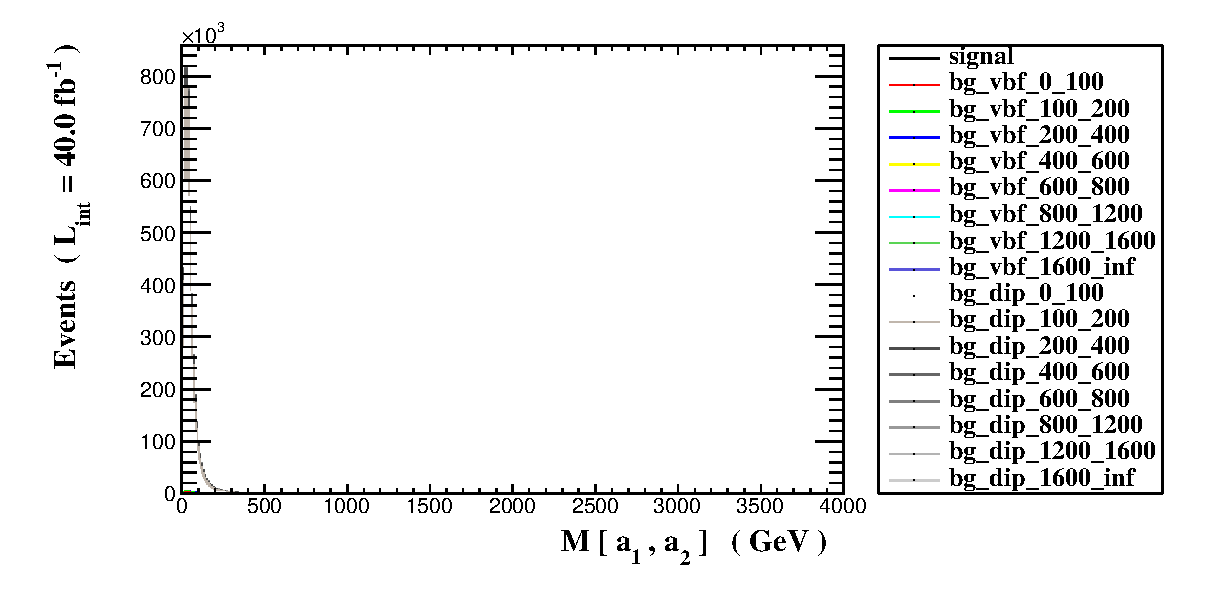
\includegraphics[scale=0.45]{selection_9.eps}\\
\caption{   }
  \end{center}
\end{figure}
      \newpage
\subsection{ Histogram 11}

\textbf{* Plot: PT ( a[1] ) }\\
   \begin{table}[H]
  \begin{center}
    \begin{tabular}{|m{23.0mm}|m{23.0mm}|m{18.0mm}|m{19.0mm}|m{19.0mm}|m{19.0mm}|m{19.0mm}|}
      \hline
      {\cellcolor{yellow}         Dataset}& {\cellcolor{yellow}         Integral}& {\cellcolor{yellow}         Entries per event}& {\cellcolor{yellow}         Mean}& {\cellcolor{yellow}         RMS}& {\cellcolor{yellow}         \% underflow}& {\cellcolor{yellow}         \% overflow}\\
      \hline
      {\cellcolor{white}         signal}& {\cellcolor{white}         4094}& {\cellcolor{white}         1.0}& {\cellcolor{white}         588.092}& {\cellcolor{white}         368.7}& {\cellcolor{green}         0.0}& {\cellcolor{green}         0.4184}\\
      \hline
      {\cellcolor{white}         bg\_vbf\_0\_100}& {\cellcolor{white}         12150}& {\cellcolor{white}         1.0}& {\cellcolor{white}         29.2182}& {\cellcolor{white}         18.35}& {\cellcolor{green}         0.0}& {\cellcolor{green}         0.0}\\
      \hline
      {\cellcolor{white}         bg\_vbf\_100\_200}& {\cellcolor{white}         9695}& {\cellcolor{white}         1.0}& {\cellcolor{white}         49.5585}& {\cellcolor{white}         34.8}& {\cellcolor{green}         0.0}& {\cellcolor{green}         0.0}\\
      \hline
      {\cellcolor{white}         bg\_vbf\_200\_400}& {\cellcolor{white}         5413}& {\cellcolor{white}         1.0}& {\cellcolor{white}         73.7805}& {\cellcolor{white}         63.02}& {\cellcolor{green}         0.0}& {\cellcolor{green}         0.0}\\
      \hline
      {\cellcolor{white}         bg\_vbf\_400\_600}& {\cellcolor{white}         986}& {\cellcolor{white}         1.0}& {\cellcolor{white}         107.933}& {\cellcolor{white}         105.3}& {\cellcolor{green}         0.0}& {\cellcolor{green}         0.0}\\
      \hline
      {\cellcolor{white}         bg\_vbf\_600\_800}& {\cellcolor{white}         252}& {\cellcolor{white}         1.0}& {\cellcolor{white}         132.767}& {\cellcolor{white}         142.4}& {\cellcolor{green}         0.0}& {\cellcolor{green}         0.0}\\
      \hline
      {\cellcolor{white}         bg\_vbf\_800\_1200}& {\cellcolor{white}         114}& {\cellcolor{white}         1.0}& {\cellcolor{white}         154.271}& {\cellcolor{white}         182.2}& {\cellcolor{green}         0.0}& {\cellcolor{green}         0.0}\\
      \hline
      {\cellcolor{white}         bg\_vbf\_1200\_1600}& {\cellcolor{white}         20.6}& {\cellcolor{white}         1.0}& {\cellcolor{white}         172.927}& {\cellcolor{white}         223.8}& {\cellcolor{green}         0.0}& {\cellcolor{green}         0.0008386}\\
      \hline
      {\cellcolor{white}         bg\_vbf\_1600\_inf}& {\cellcolor{white}         7.66}& {\cellcolor{white}         1.0}& {\cellcolor{white}         181.168}& {\cellcolor{white}         246.2}& {\cellcolor{green}         0.0}& {\cellcolor{green}         0.07471}\\
      \hline
      {\cellcolor{white}         bg\_dip\_0\_100}& {\cellcolor{white}         2710844}& {\cellcolor{white}         1.0}& {\cellcolor{white}         29.8081}& {\cellcolor{white}         19.13}& {\cellcolor{green}         0.0}& {\cellcolor{green}         0.0}\\
      \hline
      {\cellcolor{white}         bg\_dip\_100\_200}& {\cellcolor{white}         1095361}& {\cellcolor{white}         1.0}& {\cellcolor{white}         46.2821}& {\cellcolor{white}         35.82}& {\cellcolor{green}         0.0}& {\cellcolor{green}         0.0}\\
      \hline
      {\cellcolor{white}         bg\_dip\_200\_400}& {\cellcolor{white}         239548}& {\cellcolor{white}         1.0}& {\cellcolor{white}         70.6716}& {\cellcolor{white}         67.58}& {\cellcolor{green}         0.0}& {\cellcolor{green}         0.0}\\
      \hline
      {\cellcolor{white}         bg\_dip\_400\_600}& {\cellcolor{white}         28798}& {\cellcolor{white}         1.0}& {\cellcolor{white}         97.6941}& {\cellcolor{white}         110.3}& {\cellcolor{green}         0.0}& {\cellcolor{green}         0.0}\\
      \hline
      {\cellcolor{white}         bg\_dip\_600\_800}& {\cellcolor{white}         6674}& {\cellcolor{white}         1.0}& {\cellcolor{white}         114.634}& {\cellcolor{white}         141.7}& {\cellcolor{green}         0.0}& {\cellcolor{green}         0.0}\\
      \hline
      {\cellcolor{white}         bg\_dip\_800\_1200}& {\cellcolor{white}         2942}& {\cellcolor{white}         1.0}& {\cellcolor{white}         127.334}& {\cellcolor{white}         169.6}& {\cellcolor{green}         0.0}& {\cellcolor{green}         9.616e-05}\\
      \hline
      {\cellcolor{white}         bg\_dip\_1200\_1600}& {\cellcolor{white}         513}& {\cellcolor{white}         1.0}& {\cellcolor{white}         138.818}& {\cellcolor{white}         193.7}& {\cellcolor{green}         0.0}& {\cellcolor{green}         0.0002954}\\
      \hline
      {\cellcolor{white}         bg\_dip\_1600\_inf}& {\cellcolor{white}         187}& {\cellcolor{white}         1.0}& {\cellcolor{white}         146.263}& {\cellcolor{white}         199.0}& {\cellcolor{green}         0.0}& {\cellcolor{green}         0.04173}\\
\hline
    \end{tabular}
  \end{center}
\end{table}

\begin{figure}[H]
  \begin{center}
    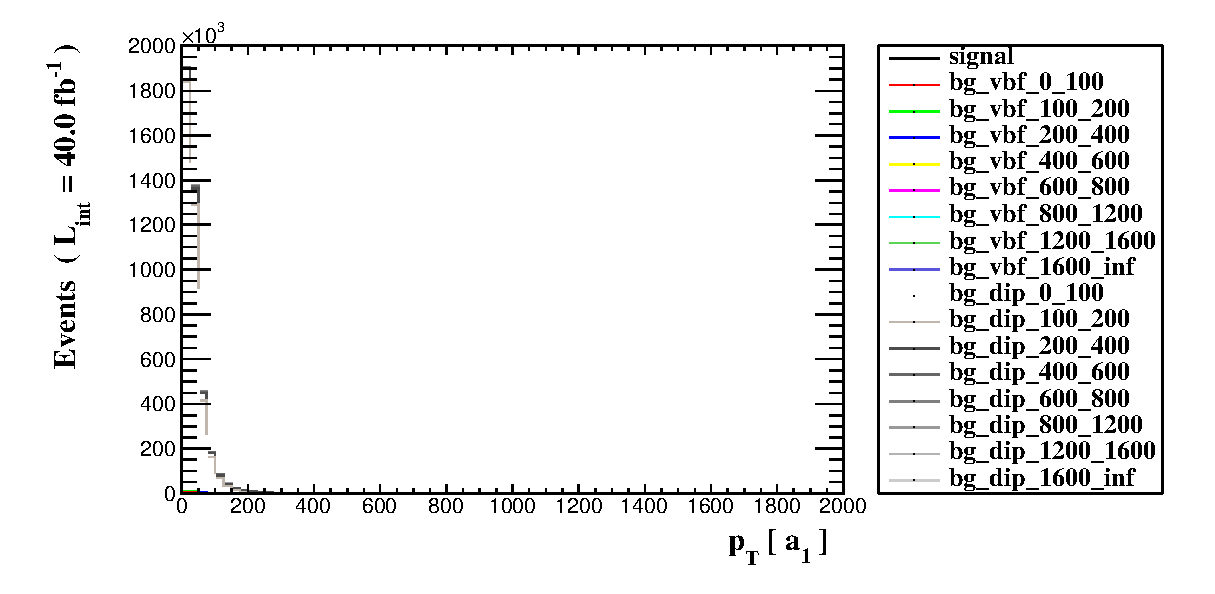
\includegraphics[scale=0.45]{selection_10.eps}\\
\caption{   }
  \end{center}
\end{figure}
      \newpage
\subsection{ Histogram 12}

\textbf{* Plot: PT ( a[2] ) }\\
   \begin{table}[H]
  \begin{center}
    \begin{tabular}{|m{23.0mm}|m{23.0mm}|m{18.0mm}|m{19.0mm}|m{19.0mm}|m{19.0mm}|m{19.0mm}|}
      \hline
      {\cellcolor{yellow}         Dataset}& {\cellcolor{yellow}         Integral}& {\cellcolor{yellow}         Entries per event}& {\cellcolor{yellow}         Mean}& {\cellcolor{yellow}         RMS}& {\cellcolor{yellow}         \% underflow}& {\cellcolor{yellow}         \% overflow}\\
      \hline
      {\cellcolor{white}         signal}& {\cellcolor{white}         4094}& {\cellcolor{white}         1.0}& {\cellcolor{white}         334.941}& {\cellcolor{white}         290.0}& {\cellcolor{green}         0.0}& {\cellcolor{green}         0.1287}\\
      \hline
      {\cellcolor{white}         bg\_vbf\_0\_100}& {\cellcolor{white}         12150}& {\cellcolor{white}         1.0}& {\cellcolor{white}         16.7975}& {\cellcolor{white}         10.54}& {\cellcolor{green}         0.0}& {\cellcolor{green}         0.0}\\
      \hline
      {\cellcolor{white}         bg\_vbf\_100\_200}& {\cellcolor{white}         9695}& {\cellcolor{white}         1.0}& {\cellcolor{white}         21.7009}& {\cellcolor{white}         16.69}& {\cellcolor{green}         0.0}& {\cellcolor{green}         0.0}\\
      \hline
      {\cellcolor{white}         bg\_vbf\_200\_400}& {\cellcolor{white}         5413}& {\cellcolor{white}         1.0}& {\cellcolor{white}         26.1576}& {\cellcolor{white}         23.66}& {\cellcolor{green}         0.0}& {\cellcolor{green}         0.0}\\
      \hline
      {\cellcolor{white}         bg\_vbf\_400\_600}& {\cellcolor{white}         986}& {\cellcolor{white}         1.0}& {\cellcolor{white}         31.3191}& {\cellcolor{white}         32.61}& {\cellcolor{green}         0.0}& {\cellcolor{green}         0.0}\\
      \hline
      {\cellcolor{white}         bg\_vbf\_600\_800}& {\cellcolor{white}         252}& {\cellcolor{white}         1.0}& {\cellcolor{white}         34.6235}& {\cellcolor{white}         38.99}& {\cellcolor{green}         0.0}& {\cellcolor{green}         0.0}\\
      \hline
      {\cellcolor{white}         bg\_vbf\_800\_1200}& {\cellcolor{white}         114}& {\cellcolor{white}         1.0}& {\cellcolor{white}         37.1184}& {\cellcolor{white}         44.65}& {\cellcolor{green}         0.0}& {\cellcolor{green}         0.0}\\
      \hline
      {\cellcolor{white}         bg\_vbf\_1200\_1600}& {\cellcolor{white}         20.6}& {\cellcolor{white}         1.0}& {\cellcolor{white}         39.4376}& {\cellcolor{white}         49.92}& {\cellcolor{green}         0.0}& {\cellcolor{green}         0.0}\\
      \hline
      {\cellcolor{white}         bg\_vbf\_1600\_inf}& {\cellcolor{white}         7.66}& {\cellcolor{white}         1.0}& {\cellcolor{white}         40.8098}& {\cellcolor{white}         52.8}& {\cellcolor{green}         0.0}& {\cellcolor{green}         0.0}\\
      \hline
      {\cellcolor{white}         bg\_dip\_0\_100}& {\cellcolor{white}         2710844}& {\cellcolor{white}         1.0}& {\cellcolor{white}         16.4095}& {\cellcolor{white}         9.466}& {\cellcolor{green}         0.0}& {\cellcolor{green}         0.0}\\
      \hline
      {\cellcolor{white}         bg\_dip\_100\_200}& {\cellcolor{white}         1095361}& {\cellcolor{white}         1.0}& {\cellcolor{white}         19.392}& {\cellcolor{white}         13.88}& {\cellcolor{green}         0.0}& {\cellcolor{green}         0.0}\\
      \hline
      {\cellcolor{white}         bg\_dip\_200\_400}& {\cellcolor{white}         239548}& {\cellcolor{white}         1.0}& {\cellcolor{white}         23.2538}& {\cellcolor{white}         20.42}& {\cellcolor{green}         0.0}& {\cellcolor{green}         0.0}\\
      \hline
      {\cellcolor{white}         bg\_dip\_400\_600}& {\cellcolor{white}         28798}& {\cellcolor{white}         1.0}& {\cellcolor{white}         27.0718}& {\cellcolor{white}         27.59}& {\cellcolor{green}         0.0}& {\cellcolor{green}         0.0}\\
      \hline
      {\cellcolor{white}         bg\_dip\_600\_800}& {\cellcolor{white}         6674}& {\cellcolor{white}         1.0}& {\cellcolor{white}         29.4856}& {\cellcolor{white}         32.31}& {\cellcolor{green}         0.0}& {\cellcolor{green}         0.0}\\
      \hline
      {\cellcolor{white}         bg\_dip\_800\_1200}& {\cellcolor{white}         2942}& {\cellcolor{white}         1.0}& {\cellcolor{white}         31.4354}& {\cellcolor{white}         36.1}& {\cellcolor{green}         0.0}& {\cellcolor{green}         0.0}\\
      \hline
      {\cellcolor{white}         bg\_dip\_1200\_1600}& {\cellcolor{white}         513}& {\cellcolor{white}         1.0}& {\cellcolor{white}         33.6499}& {\cellcolor{white}         39.8}& {\cellcolor{green}         0.0}& {\cellcolor{green}         0.0}\\
      \hline
      {\cellcolor{white}         bg\_dip\_1600\_inf}& {\cellcolor{white}         187}& {\cellcolor{white}         1.0}& {\cellcolor{white}         35.6026}& {\cellcolor{white}         42.32}& {\cellcolor{green}         0.0}& {\cellcolor{green}         0.0}\\
\hline
    \end{tabular}
  \end{center}
\end{table}

\begin{figure}[H]
  \begin{center}
    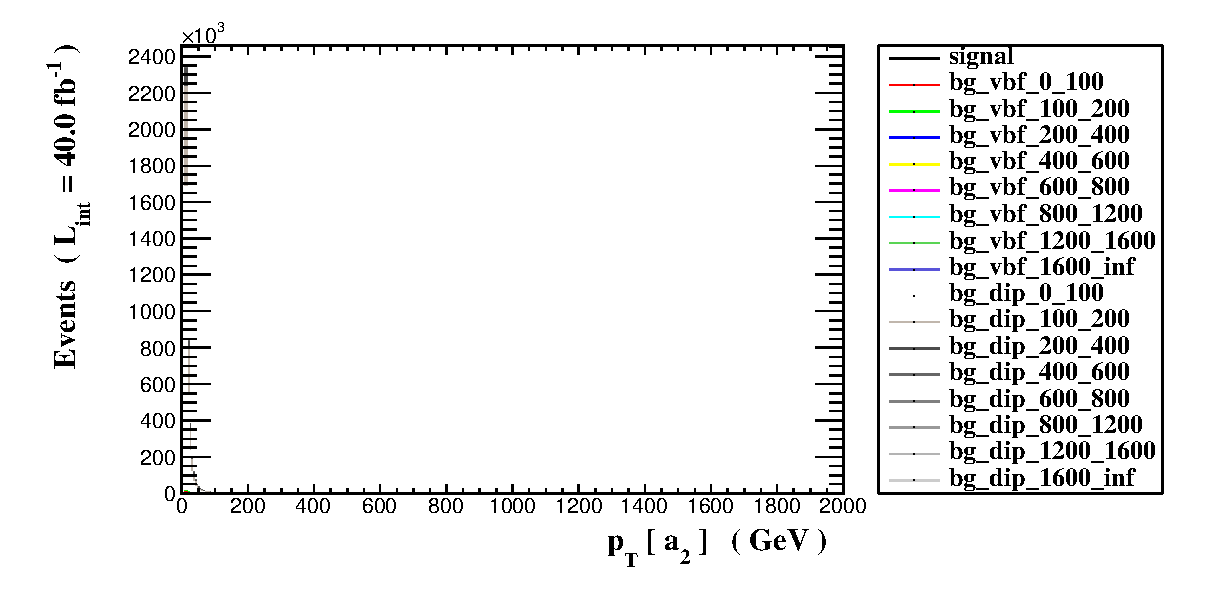
\includegraphics[scale=0.45]{selection_11.eps}\\
\caption{   }
  \end{center}
\end{figure}
      \newpage
\subsection{ Histogram 13}

\textbf{* Plot: THT}\\
   \begin{table}[H]
  \begin{center}
    \begin{tabular}{|m{23.0mm}|m{23.0mm}|m{18.0mm}|m{19.0mm}|m{19.0mm}|m{19.0mm}|m{19.0mm}|}
      \hline
      {\cellcolor{yellow}         Dataset}& {\cellcolor{yellow}         Integral}& {\cellcolor{yellow}         Entries per event}& {\cellcolor{yellow}         Mean}& {\cellcolor{yellow}         RMS}& {\cellcolor{yellow}         \% underflow}& {\cellcolor{yellow}         \% overflow}\\
      \hline
      {\cellcolor{white}         signal}& {\cellcolor{white}         4094}& {\cellcolor{white}         1.0}& {\cellcolor{white}         607.684}& {\cellcolor{white}         391.1}& {\cellcolor{green}         0.0}& {\cellcolor{green}         0.0}\\
      \hline
      {\cellcolor{white}         bg\_vbf\_0\_100}& {\cellcolor{white}         12150}& {\cellcolor{white}         1.0}& {\cellcolor{white}         73.0879}& {\cellcolor{white}         14.72}& {\cellcolor{green}         0.0}& {\cellcolor{green}         0.0}\\
      \hline
      {\cellcolor{white}         bg\_vbf\_100\_200}& {\cellcolor{white}         9695}& {\cellcolor{white}         1.0}& {\cellcolor{white}         142.161}& {\cellcolor{white}         28.33}& {\cellcolor{green}         0.0}& {\cellcolor{green}         0.0}\\
      \hline
      {\cellcolor{white}         bg\_vbf\_200\_400}& {\cellcolor{white}         5413}& {\cellcolor{white}         1.0}& {\cellcolor{white}         270.622}& {\cellcolor{white}         53.34}& {\cellcolor{green}         0.0}& {\cellcolor{green}         0.0}\\
      \hline
      {\cellcolor{white}         bg\_vbf\_400\_600}& {\cellcolor{white}         986}& {\cellcolor{white}         1.0}& {\cellcolor{white}         475.894}& {\cellcolor{white}         55.07}& {\cellcolor{green}         0.0}& {\cellcolor{green}         0.0}\\
      \hline
      {\cellcolor{white}         bg\_vbf\_600\_800}& {\cellcolor{white}         252}& {\cellcolor{white}         1.0}& {\cellcolor{white}         680.199}& {\cellcolor{white}         56.48}& {\cellcolor{green}         0.0}& {\cellcolor{green}         0.0}\\
      \hline
      {\cellcolor{white}         bg\_vbf\_800\_1200}& {\cellcolor{white}         114}& {\cellcolor{white}         1.0}& {\cellcolor{white}         938.845}& {\cellcolor{white}         110.2}& {\cellcolor{green}         0.0}& {\cellcolor{green}         0.0}\\
      \hline
      {\cellcolor{white}         bg\_vbf\_1200\_1600}& {\cellcolor{white}         20.6}& {\cellcolor{white}         1.0}& {\cellcolor{white}         1349.44}& {\cellcolor{white}         125.4}& {\cellcolor{green}         0.0}& {\cellcolor{green}         0.0}\\
      \hline
      {\cellcolor{white}         bg\_vbf\_1600\_inf}& {\cellcolor{white}         7.66}& {\cellcolor{white}         1.0}& {\cellcolor{white}         1929.14}& {\cellcolor{white}         471.8}& {\cellcolor{green}         0.0}& {\cellcolor{green}         0.273}\\
      \hline
      {\cellcolor{white}         bg\_dip\_0\_100}& {\cellcolor{white}         2710847}& {\cellcolor{white}         1.0}& {\cellcolor{white}         68.539}& {\cellcolor{white}         15.42}& {\cellcolor{green}         0.0}& {\cellcolor{green}         0.0}\\
      \hline
      {\cellcolor{white}         bg\_dip\_100\_200}& {\cellcolor{white}         1095362}& {\cellcolor{white}         1.0}& {\cellcolor{white}         133.772}& {\cellcolor{white}         26.41}& {\cellcolor{green}         0.0}& {\cellcolor{green}         0.0}\\
      \hline
      {\cellcolor{white}         bg\_dip\_200\_400}& {\cellcolor{white}         239548}& {\cellcolor{white}         1.0}& {\cellcolor{white}         261.481}& {\cellcolor{white}         50.79}& {\cellcolor{green}         0.0}& {\cellcolor{green}         0.0}\\
      \hline
      {\cellcolor{white}         bg\_dip\_400\_600}& {\cellcolor{white}         28798}& {\cellcolor{white}         1.0}& {\cellcolor{white}         473.915}& {\cellcolor{white}         54.57}& {\cellcolor{green}         0.0}& {\cellcolor{green}         0.0}\\
      \hline
      {\cellcolor{white}         bg\_dip\_600\_800}& {\cellcolor{white}         6674}& {\cellcolor{white}         1.0}& {\cellcolor{white}         679.837}& {\cellcolor{white}         55.82}& {\cellcolor{green}         0.0}& {\cellcolor{green}         0.0}\\
      \hline
      {\cellcolor{white}         bg\_dip\_800\_1200}& {\cellcolor{white}         2942}& {\cellcolor{white}         1.0}& {\cellcolor{white}         939.589}& {\cellcolor{white}         106.7}& {\cellcolor{green}         0.0}& {\cellcolor{green}         0.0}\\
      \hline
      {\cellcolor{white}         bg\_dip\_1200\_1600}& {\cellcolor{white}         513}& {\cellcolor{white}         1.0}& {\cellcolor{white}         1351.79}& {\cellcolor{white}         111.6}& {\cellcolor{green}         0.0}& {\cellcolor{green}         0.0}\\
      \hline
      {\cellcolor{white}         bg\_dip\_1600\_inf}& {\cellcolor{white}         187}& {\cellcolor{white}         1.0}& {\cellcolor{white}         1962.18}& {\cellcolor{white}         387.0}& {\cellcolor{green}         0.0}& {\cellcolor{green}         0.2515}\\
\hline
    \end{tabular}
  \end{center}
\end{table}

\begin{figure}[H]
  \begin{center}
    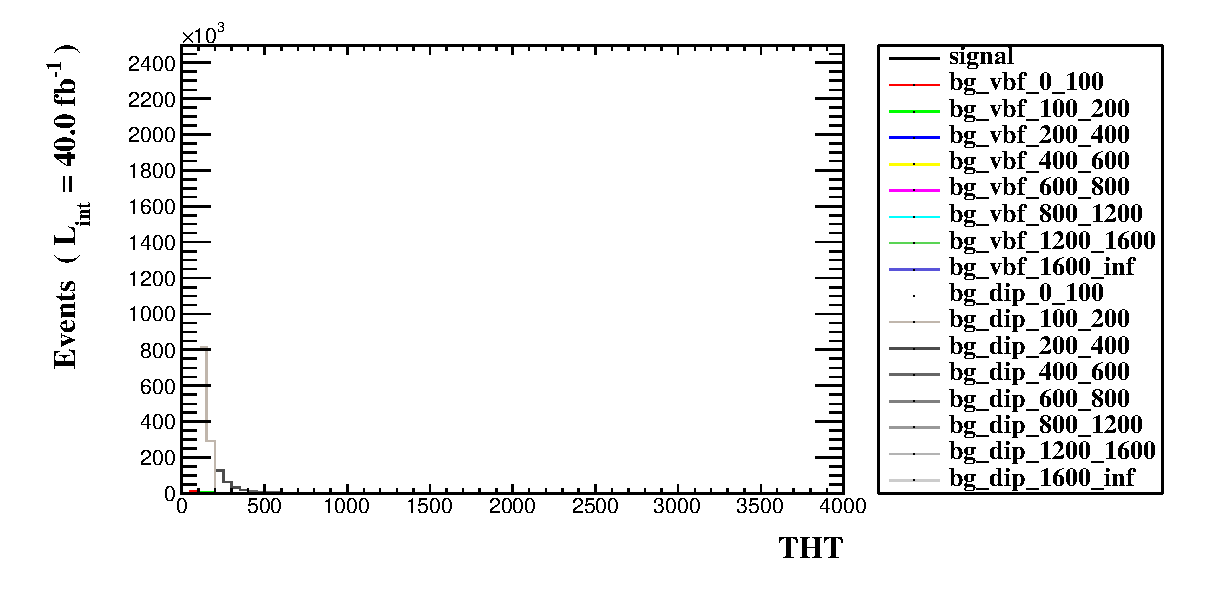
\includegraphics[scale=0.45]{selection_12.eps}\\
\caption{   }
  \end{center}
\end{figure}
      \newpage
\subsection{ Histogram 14}

\textbf{* Plot: MET}\\
   \begin{table}[H]
  \begin{center}
    \begin{tabular}{|m{23.0mm}|m{23.0mm}|m{18.0mm}|m{19.0mm}|m{19.0mm}|m{19.0mm}|m{19.0mm}|}
      \hline
      {\cellcolor{yellow}         Dataset}& {\cellcolor{yellow}         Integral}& {\cellcolor{yellow}         Entries per event}& {\cellcolor{yellow}         Mean}& {\cellcolor{yellow}         RMS}& {\cellcolor{yellow}         \% underflow}& {\cellcolor{yellow}         \% overflow}\\
      \hline
      {\cellcolor{white}         signal}& {\cellcolor{white}         4094}& {\cellcolor{white}         1.0}& {\cellcolor{white}         8.33075e-09}& {\cellcolor{white}         1.078e-08}& {\cellcolor{green}         0.0}& {\cellcolor{green}         0.0}\\
      \hline
      {\cellcolor{white}         bg\_vbf\_0\_100}& {\cellcolor{white}         12150}& {\cellcolor{white}         1.0}& {\cellcolor{white}         5.87589e-10}& {\cellcolor{white}         4.167e-10}& {\cellcolor{green}         0.0}& {\cellcolor{green}         0.0}\\
      \hline
      {\cellcolor{white}         bg\_vbf\_100\_200}& {\cellcolor{white}         9695}& {\cellcolor{white}         1.0}& {\cellcolor{white}         9.77311e-10}& {\cellcolor{white}         1.133e-09}& {\cellcolor{green}         0.0}& {\cellcolor{green}         0.0}\\
      \hline
      {\cellcolor{white}         bg\_vbf\_200\_400}& {\cellcolor{white}         5413}& {\cellcolor{white}         1.0}& {\cellcolor{white}         3.24025e-09}& {\cellcolor{white}         2.224e-09}& {\cellcolor{green}         0.0}& {\cellcolor{green}         0.0}\\
      \hline
      {\cellcolor{white}         bg\_vbf\_400\_600}& {\cellcolor{white}         986}& {\cellcolor{white}         1.0}& {\cellcolor{white}         4.5261e-09}& {\cellcolor{white}         2.611e-09}& {\cellcolor{green}         0.0}& {\cellcolor{green}         0.0}\\
      \hline
      {\cellcolor{white}         bg\_vbf\_600\_800}& {\cellcolor{white}         252}& {\cellcolor{white}         1.0}& {\cellcolor{white}         4.90173e-09}& {\cellcolor{white}         2.72e-09}& {\cellcolor{green}         0.0}& {\cellcolor{green}         0.0}\\
      \hline
      {\cellcolor{white}         bg\_vbf\_800\_1200}& {\cellcolor{white}         114}& {\cellcolor{white}         1.0}& {\cellcolor{white}         5.15201e-09}& {\cellcolor{white}         2.983e-09}& {\cellcolor{green}         0.0}& {\cellcolor{green}         0.0}\\
      \hline
      {\cellcolor{white}         bg\_vbf\_1200\_1600}& {\cellcolor{white}         20.6}& {\cellcolor{white}         1.0}& {\cellcolor{white}         5.8088e-09}& {\cellcolor{white}         5.344e-09}& {\cellcolor{green}         0.0}& {\cellcolor{green}         0.0}\\
      \hline
      {\cellcolor{white}         bg\_vbf\_1600\_inf}& {\cellcolor{white}         7.66}& {\cellcolor{white}         1.0}& {\cellcolor{white}         1.2815e-08}& {\cellcolor{white}         1.633e-08}& {\cellcolor{green}         0.0}& {\cellcolor{green}         0.0}\\
      \hline
      {\cellcolor{white}         bg\_dip\_0\_100}& {\cellcolor{white}         2710847}& {\cellcolor{white}         1.0}& {\cellcolor{white}         5.83304e-10}& {\cellcolor{white}         4.119e-10}& {\cellcolor{green}         0.0}& {\cellcolor{green}         0.0}\\
      \hline
      {\cellcolor{white}         bg\_dip\_100\_200}& {\cellcolor{white}         1095362}& {\cellcolor{white}         1.0}& {\cellcolor{white}         9.17249e-10}& {\cellcolor{white}         1.079e-09}& {\cellcolor{green}         0.0}& {\cellcolor{green}         0.0}\\
      \hline
      {\cellcolor{white}         bg\_dip\_200\_400}& {\cellcolor{white}         239548}& {\cellcolor{white}         1.0}& {\cellcolor{white}         3.1345e-09}& {\cellcolor{white}         2.199e-09}& {\cellcolor{green}         0.0}& {\cellcolor{green}         0.0}\\
      \hline
      {\cellcolor{white}         bg\_dip\_400\_600}& {\cellcolor{white}         28798}& {\cellcolor{white}         1.0}& {\cellcolor{white}         4.43742e-09}& {\cellcolor{white}         2.58e-09}& {\cellcolor{green}         0.0}& {\cellcolor{green}         0.0}\\
      \hline
      {\cellcolor{white}         bg\_dip\_600\_800}& {\cellcolor{white}         6674}& {\cellcolor{white}         1.0}& {\cellcolor{white}         4.80256e-09}& {\cellcolor{white}         2.678e-09}& {\cellcolor{green}         0.0}& {\cellcolor{green}         0.0}\\
      \hline
      {\cellcolor{white}         bg\_dip\_800\_1200}& {\cellcolor{white}         2942}& {\cellcolor{white}         1.0}& {\cellcolor{white}         5.06408e-09}& {\cellcolor{white}         3.037e-09}& {\cellcolor{green}         0.0}& {\cellcolor{green}         0.0}\\
      \hline
      {\cellcolor{white}         bg\_dip\_1200\_1600}& {\cellcolor{white}         513}& {\cellcolor{white}         1.0}& {\cellcolor{white}         5.59027e-09}& {\cellcolor{white}         4.834e-09}& {\cellcolor{green}         0.0}& {\cellcolor{green}         0.0}\\
      \hline
      {\cellcolor{white}         bg\_dip\_1600\_inf}& {\cellcolor{white}         187}& {\cellcolor{white}         1.0}& {\cellcolor{white}         1.25054e-08}& {\cellcolor{white}         1.605e-08}& {\cellcolor{green}         0.0}& {\cellcolor{green}         0.0}\\
\hline
    \end{tabular}
  \end{center}
\end{table}

\begin{figure}[H]
  \begin{center}
    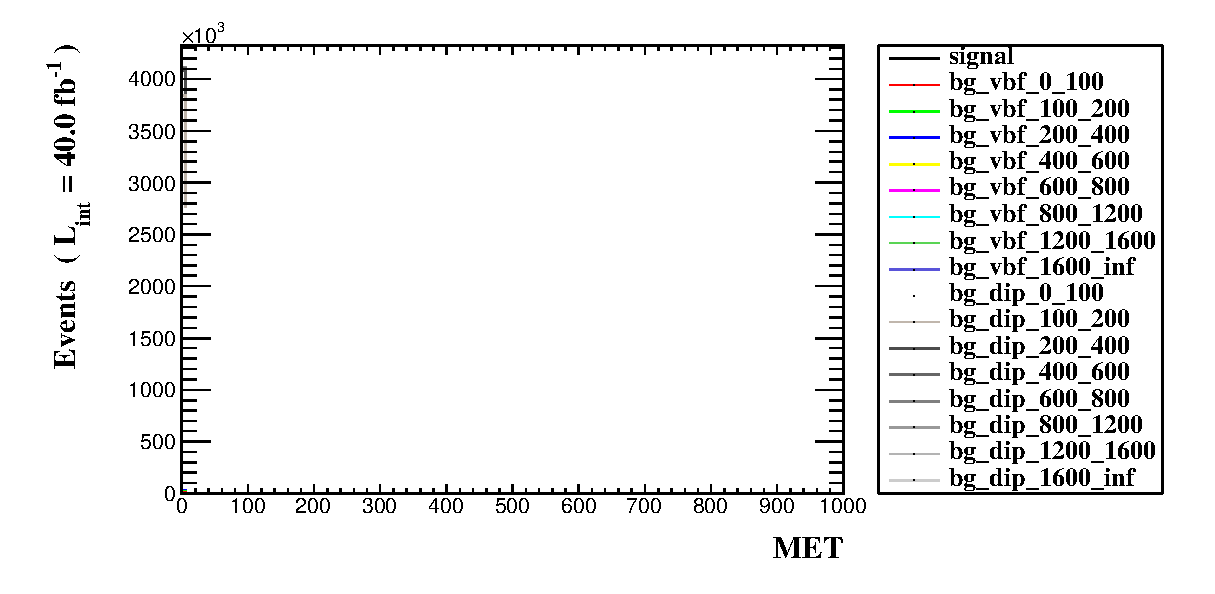
\includegraphics[scale=0.45]{selection_13.eps}\\
\caption{   }
  \end{center}
\end{figure}
      \newpage
\subsection{ Histogram 15}

\textbf{* Plot: TET}\\
   \begin{table}[H]
  \begin{center}
    \begin{tabular}{|m{23.0mm}|m{23.0mm}|m{18.0mm}|m{19.0mm}|m{19.0mm}|m{19.0mm}|m{19.0mm}|}
      \hline
      {\cellcolor{yellow}         Dataset}& {\cellcolor{yellow}         Integral}& {\cellcolor{yellow}         Entries per event}& {\cellcolor{yellow}         Mean}& {\cellcolor{yellow}         RMS}& {\cellcolor{yellow}         \% underflow}& {\cellcolor{yellow}         \% overflow}\\
      \hline
      {\cellcolor{white}         signal}& {\cellcolor{white}         4094}& {\cellcolor{white}         1.0}& {\cellcolor{white}         1530.71}& {\cellcolor{white}         825.4}& {\cellcolor{green}         0.0}& {\cellcolor{green}         0.0001}\\
      \hline
      {\cellcolor{white}         bg\_vbf\_0\_100}& {\cellcolor{white}         12150}& {\cellcolor{white}         1.0}& {\cellcolor{white}         119.104}& {\cellcolor{white}         33.34}& {\cellcolor{green}         0.0}& {\cellcolor{green}         0.0}\\
      \hline
      {\cellcolor{white}         bg\_vbf\_100\_200}& {\cellcolor{white}         9695}& {\cellcolor{white}         1.0}& {\cellcolor{white}         213.42}& {\cellcolor{white}         57.37}& {\cellcolor{green}         0.0}& {\cellcolor{green}         0.0}\\
      \hline
      {\cellcolor{white}         bg\_vbf\_200\_400}& {\cellcolor{white}         5413}& {\cellcolor{white}         1.0}& {\cellcolor{white}         370.559}& {\cellcolor{white}         100.3}& {\cellcolor{green}         0.0}& {\cellcolor{green}         0.0}\\
      \hline
      {\cellcolor{white}         bg\_vbf\_400\_600}& {\cellcolor{white}         986}& {\cellcolor{white}         1.0}& {\cellcolor{white}         615.141}& {\cellcolor{white}         138.1}& {\cellcolor{green}         0.0}& {\cellcolor{green}         0.0}\\
      \hline
      {\cellcolor{white}         bg\_vbf\_600\_800}& {\cellcolor{white}         252}& {\cellcolor{white}         1.0}& {\cellcolor{white}         847.563}& {\cellcolor{white}         173.8}& {\cellcolor{green}         0.0}& {\cellcolor{green}         0.0}\\
      \hline
      {\cellcolor{white}         bg\_vbf\_800\_1200}& {\cellcolor{white}         114}& {\cellcolor{white}         1.0}& {\cellcolor{white}         1130.07}& {\cellcolor{white}         235.9}& {\cellcolor{green}         0.0}& {\cellcolor{green}         0.0}\\
      \hline
      {\cellcolor{white}         bg\_vbf\_1200\_1600}& {\cellcolor{white}         20.6}& {\cellcolor{white}         1.0}& {\cellcolor{white}         1561.37}& {\cellcolor{white}         280.1}& {\cellcolor{green}         0.0}& {\cellcolor{green}         0.0}\\
      \hline
      {\cellcolor{white}         bg\_vbf\_1600\_inf}& {\cellcolor{white}         7.66}& {\cellcolor{white}         1.0}& {\cellcolor{white}         2146.89}& {\cellcolor{white}         558.2}& {\cellcolor{green}         0.0}& {\cellcolor{green}         0.0}\\
      \hline
      {\cellcolor{white}         bg\_dip\_0\_100}& {\cellcolor{white}         2710847}& {\cellcolor{white}         1.0}& {\cellcolor{white}         114.757}& {\cellcolor{white}         32.41}& {\cellcolor{green}         0.0}& {\cellcolor{green}         0.0}\\
      \hline
      {\cellcolor{white}         bg\_dip\_100\_200}& {\cellcolor{white}         1095362}& {\cellcolor{white}         1.0}& {\cellcolor{white}         199.446}& {\cellcolor{white}         55.32}& {\cellcolor{green}         0.0}& {\cellcolor{green}         0.0}\\
      \hline
      {\cellcolor{white}         bg\_dip\_200\_400}& {\cellcolor{white}         239548}& {\cellcolor{white}         1.0}& {\cellcolor{white}         355.406}& {\cellcolor{white}         98.44}& {\cellcolor{green}         0.0}& {\cellcolor{green}         0.0}\\
      \hline
      {\cellcolor{white}         bg\_dip\_400\_600}& {\cellcolor{white}         28798}& {\cellcolor{white}         1.0}& {\cellcolor{white}         598.681}& {\cellcolor{white}         138.0}& {\cellcolor{green}         0.0}& {\cellcolor{green}         0.0}\\
      \hline
      {\cellcolor{white}         bg\_dip\_600\_800}& {\cellcolor{white}         6674}& {\cellcolor{white}         1.0}& {\cellcolor{white}         823.955}& {\cellcolor{white}         168.1}& {\cellcolor{green}         0.0}& {\cellcolor{green}         0.0}\\
      \hline
      {\cellcolor{white}         bg\_dip\_800\_1200}& {\cellcolor{white}         2942}& {\cellcolor{white}         1.0}& {\cellcolor{white}         1098.36}& {\cellcolor{white}         217.0}& {\cellcolor{green}         0.0}& {\cellcolor{green}         0.0}\\
      \hline
      {\cellcolor{white}         bg\_dip\_1200\_1600}& {\cellcolor{white}         513}& {\cellcolor{white}         1.0}& {\cellcolor{white}         1524.22}& {\cellcolor{white}         240.1}& {\cellcolor{green}         0.0}& {\cellcolor{green}         0.0}\\
      \hline
      {\cellcolor{white}         bg\_dip\_1600\_inf}& {\cellcolor{white}         187}& {\cellcolor{white}         1.0}& {\cellcolor{white}         2144.01}& {\cellcolor{white}         446.2}& {\cellcolor{green}         0.0}& {\cellcolor{green}         0.0}\\
\hline
    \end{tabular}
  \end{center}
\end{table}

\begin{figure}[H]
  \begin{center}
    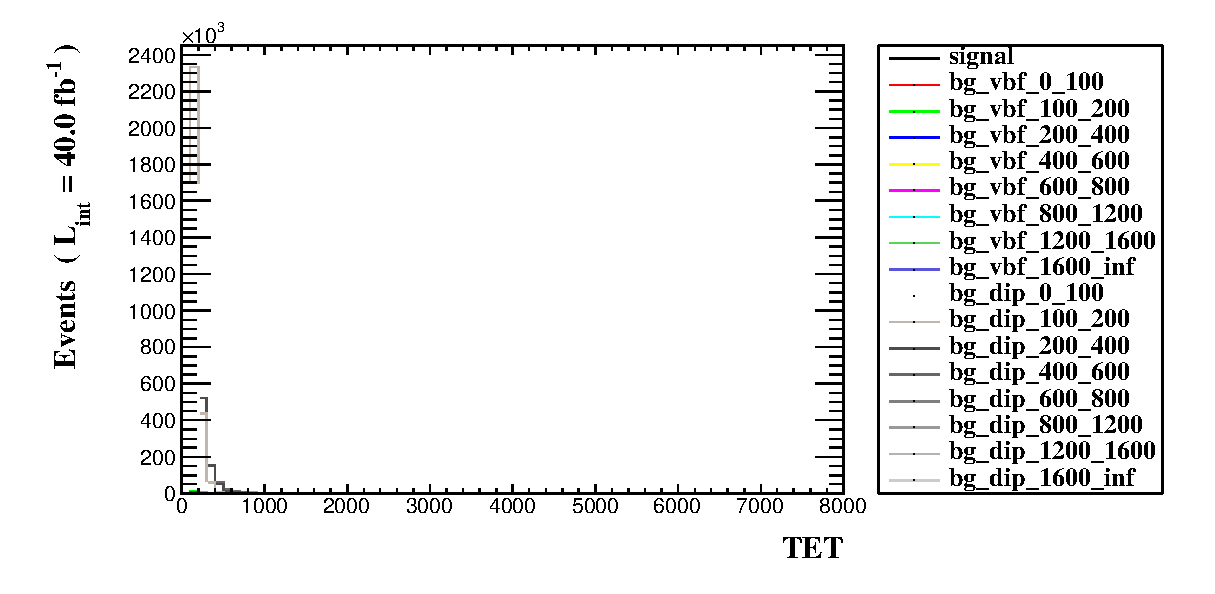
\includegraphics[scale=0.45]{selection_14.eps}\\
\caption{   }
  \end{center}
\end{figure}
      \end{document}
